
\begin{algorithm}[t]
\caption{Meta-chain Distillation}
\label{alg:distill}
\begin{algorithmic}[1]
\STATE set $S_\circ=\varnothing$, $\bZ^{(0)}=\boldsymbol{0}$, $\iota(x)=0$ for all $x\in S$,
\STATE $T_{\dist}=O(M^2(\log K)^2\ep^{-2})$, $T_{\thres}=\widetilde{O}(M\ep^{-1})$
\STATE $\eta=\Theta(K)$, $\beta=\Theta(\log (M/\ep))$
\WHILE[cluster labeling]{$\iota^{-1}(0)\ne\varnothing$}
\STATE draw $X_0\in\iota^{-1}(0)$
\STATE $S_\circ\gets S_\circ\cup\{X_0\}$, $\iota(X_0)\gets X_0$
\FOR{$t=1,\cdots,T_0$}
\STATE generate $X_t^\ep\sim p^\ep(\cdot|X_{t-1}^\ep)$
\STATE $\iota(X_t^\ep)\gets X_0$
\ENDFOR
\ENDWHILE

\FOR[data collection]{$t=1,2,\cdots$}
\IF{$X_t^\ep\in S_\circ$}
\STATE $Y_0^{(t)}, Y_1^{(t_{\prev})}\gets X_t^\ep$
\STATE $t_{\prev}\gets t$
\ELSE
\STATE $Y_0^{(t)},Y_1^{(t)}\gets \iota(X_t^\ep)$
\ENDIF
\ENDFOR

\FOR[distillation]{$t=1,\cdots,T_{\dist}$}
\STATE $\bZ^{(t)} = \bZ^{(t-1)} - \eta\nabla \EE{Y_0,Y_1}{-\log\hat{p}_{\bZ^{(t-1)}}(Y_1|Y_0)}$
\IF{$t=T_{\thres}$}
\STATE $z_{k\ell}^{(T_{\thres})} \gets -\infty$ if $\hat{q}_{k\ell}^{(T_{\thres})} < c_{\thres}\ep/M$
\ENDIF
\ENDFOR

\STATE $\bz_{k\ell}^+ \gets \bz_{k\ell}^{(T_{\dist})} + \beta$ for $\ell\ne k$ \COMMENT{time rescaling}
\STATE return $\bZ^+$
\end{algorithmic}
\end{algorithm}

\bigskip 

\section{Additional Related Works}\label{app:related}

\paragraph{Theoretical Analysis of CoT.} Some theoretical works have focused on the expressivity of CoT \citep{Feng23,merrill2023expresssive,Chiang23,li2024chain}, analysis of optimization and estimation ability \citep{Li24how,Hu24,kim2024transformers}, or in-context learning ability \citep{Li23,Satwik24}. More closely related to our paper, \citet{sanford24log,sanford2024understanding, abbe2024far} study the algorithmic reasoning capabilities of CoT or scratchpad transformers for certain computational or graph-based tasks. Also, \citet{Nichani24} analyze how simple transformer models learn latent causal structure within the data.

\paragraph{LLMs as Markov processes.} \citet{Zekri24} study the equivalence between autoregressive models and general length Markov chains. \citet{Makkuva24,Edelman24} model sequential data as a Markov chain and analyze the properties of a single-layer transformer. \citet{Ildiz24} establish a link between self-attention and context-conditioned Markov models. Such works generally focus on interpreting next-token prediction of a specific architecture, and do not consider the abstraction to CoT reasoning.

\paragraph{Metastable Markov chains.}
The literature on metastable Markov processes is vast \citep[e.g.,][]{Madras01,Bovier02,Beltran11,Landim18}. Here we only mention the results most relevant to our theory. In particular, as reversibility is unrealistic to presume for language or reasoning models, we generally restrict our attention to works on nonreversible processes. \citet{Fritzsche08,Jacobi10,Tifenbach11,Fackeldey18} study various spectral methods to identify metastable states of Markov chains. \citet{Landim12, Cirillo14,Fernandez14,Fernandez16,Bianchi16} analyze critical configurations and escape times for metastable dynamics, while \citet{Landim15} propose a recursive procedure for model reduction. Most relevant to our work, \citet{Wicks05,Betz16} give a complete hierarchical characterization of the effective dynamics of perturbed chains but only in the asymptotic limit; building on their results, we develop a new quantitative perturbation analysis throughout Appendix \ref{app:perturb}.

\section{Preliminaries}\label{app:prelim}

\subsection{Pseudo-Spectral Gap and Mixing}

By taking Assumption \ref{ass:sparse} and multiplying $\ep$ by a constant if necessary, we assume that $c\ep\le p^\ep(y|x)\le\ep$ for some $c>0$ and all $(x,y)\in E_s$ throughout the appendix.

\begin{defn}[mixing time]
For a time-homogeneous ergodic Markov chain $X=(X_t)_{t\ge 0}$ on a finite state space $\Omega$ with transition kernel $p$ and stationary distribution $\pi$, the mixing time $t_{\mix}$ is defined as
\begin{equation*}
t_{\mix}(\epsilon) = \min\left\{t\ge 0: \forall s\ge t,\; \sup_{x\in\Omega}\norm{p^s(\cdot|x) - \pi}_{\TV} \le\epsilon \right\}.
\end{equation*}
\end{defn}

\begin{defn}[hitting and return times]
The $n$th \emph{hitting time} and \emph{return time} of $X^\ep$ to a set $A\subseteq S$ for $n\in\NN$ are defined as
\begin{align*}
\tau_{A,n}^\ep &= \inf\{t\ge 0:\abs{\{0\le t'\le t: X_{t'}^\ep\in A\}}=n\},\\
\bar{\tau}_{A,n}^\ep &= \inf\{t> 0:\abs{\{0<t'\le t: X_{t'}^\ep\in A\}}=n\}.
\end{align*}
In particular, we write $\tau_A^\ep = \tau_{A,1}^\ep$ and $\bar{\tau}_A^\ep = \bar{\tau}_{A,1}^\ep$. We write $\tau_x^\ep=\tau_{\{x\}}^\ep$, etc. for simplicity.
\end{defn}

The chain $X$ is \emph{reversible} if it satisfies the \emph{detailed balance equation}
\begin{equation*}
\pi(x) p(y|x) = \pi(y) p(x|y) \quad\forall x,y\in\Omega.
\end{equation*}
While we do not assume reversibility in this paper, it is informative to compare the conditions for rapid mixing. Denote the transition matrix corresponding to $p$ by $\bP$ and let the eigenvalues of $\bP$ ordered by absolute value be $1=\lambda_1(\bP)\ge |\lambda_2(\bP)|\ge |\lambda_3(\bP)|\ge\cdots$. For reversible chains, all eigenvalues are real and the mixing time is closely governed by the (absolute) spectral gap $\gamma(\bP) = 1-|\lambda_2(\bP)|$ \citep{Levin09}:
\begin{equation*}
\frac{1}{2\log 2\epsilon} \left(\frac{1}{\gamma(\bP)}-1\right) \le t_{\mix}(\epsilon) \le \frac{1}{\gamma(\bP)} \log\frac{1}{\pi_*\epsilon},
\end{equation*}
where $\pi_* = \min_{x\in\Omega}\pi(x)$ is the minimum stationary probability.

For nonreversible chains, the analogous quantity to $\gamma(\bP)$ is given by the \emph{pseudo-spectral gap}:

\begin{defn}[\citet{Paulin15}]
The \emph{pseudo-spectral gap} of $\bP$ is given as
\begin{equation*}
\gamma^\dagger(\bP) := \max_{m\in\NN} \frac{\gamma((\bP^\dagger)^m \bP^m)}{m}
\end{equation*}
where $\bP^\dagger$ is the time reversal of $\bP$, defined as $\bP^\dagger_{ij} = \pi_j \bP_{ji}/\pi_i$.
\end{defn}

When $X$ is reversible, it holds that $\gamma(\bP)\le\gamma^\dagger(\bP)\le 2\gamma(\bP)$ \citep[Lemma 15]{Wolfer22}. Moreover, $\gamma^\dagger(\bP)$ controls the mixing time similarly to $\gamma(\bP)$:

\begin{prop}[\citet{Paulin15}, Proposition 3.4]\label{thm:psmix}
For $0<\epsilon<1$,
\begin{equation*}
\frac{1-2\epsilon}{\gamma^\dagger(\bP)} \le t_{\mix}(\epsilon) \le \frac{1}{\gamma^\dagger(\bP)} \left(1+2\log\frac{1}{2\epsilon} +\log\frac{1}{\pi_*}\right).
\end{equation*}
\end{prop}

Denote the maximum row sum norm as $\norm{\bA}_{1,\infty} = \max_i\sum_j |a_{ij}|$ for $\bA=(a_{ij})$.
\begin{lemma}\label{thm:12norm}
For $\bA\in\RR^{m\times m}$ it holds that $\norm{\bA}_2 \le\sqrt{m} \norm{\bA}_{1,\infty}$.
\end{lemma}

\begin{proof}
For arbitrary $v\in\RR^m$ with $\norm{v}=1$,
\begin{align*}
\norm{\bA v}^2 = \sum_i\left(\sum_j a_{ij}v_j\right)^2 \le \sum_i \sum_j a_{ij}^2 \le \sum_i\left(\sum_j |a_{ij}|\right)^2 \le m\norm{\bA}_{1,\infty}^2.
\end{align*}
\end{proof}

\subsection{Stochastic Complementation}\label{sec:stocomp}

We denote the stochastic block matrix $\bP^\ep$ corresponding to the kernel $p^\ep$ and partition $S=\cup_{k=1}^K C_k$ as
\begin{align*}
\bP^\ep = \begin{pmatrix}
\bP_{11}^\ep &\cdots & \bP_{1K}^\ep\\
\vdots& \ddots &\vdots\\
\bP_{K1}^\ep &\cdots & \bP_{KK}^\ep
\end{pmatrix}.
\end{align*}
That is, the probability $p^\ep(y|x)$ is contained in the $(x,y)$ component, and the rows of $\bP^\ep$ all sum to $1$. The \textit{stochastic complement} of $\bP_{kk}^\ep$ is defined as \citep{Meyer89}
\begin{equation*}
\bS_{kk}^\ep = \bP_{kk}^\ep + \bP_{k*}^\ep(\bI-\bP_k^\ep)^{-1} \bP_{*k}^\ep
\end{equation*}
where $\bP_{k*}^\ep$ is the $k$th block row of $\bP^\ep$ with $\bP_{kk}^\ep$ removed; $\bP_{*k}^\ep$ is the $k$th block column of $\bP^\ep$ with $\bP_{kk}^\ep$ removed; and $\bP_k^\ep$ is the principal block submatrix of $\bP^\ep$ with the $k$th row and column removed. When $\ep=0$, it follows that $\bP_{ij}^0=\boldsymbol{0}$ when $i\neq j$ and $\bS_{kk}^0 = \bP_{kk}^0$ is the transition matrix of $p^0$ restricted to $C_k$.

The following results are fundamental to the theory of stochastic complementation.

\begin{thm}[\citet{Meyer89}, Theorem 2.3]\label{thm:complement}
If $\bP^\ep$ is an irreducible stochastic matrix for $\ep>0$, each stochastic complement $\bS_{kk}^\ep$ is also an irreducible stochastic matrix. Moreover, $\bS_{kk}^\ep$ is equal to the transition matrix of the reduced chain $\tilde{X}^{k,\ep}$ on $C_k$,
\begin{equation}\label{eq:reduced}
\tilde{X}_t^{k,\ep} := X_{\tau_{C_k,t+1}^\ep}^\ep, \quad t\in\NN_0
\end{equation}
obtained from $X^\ep$ by deleting transitions to states outside of $C_k$.
\end{thm}

We further denote the transition kernel of $\tilde{X}_t^{k,\ep}$ corresponding to $\bS_{kk}^\ep$ as $s_{kk}^\ep$, so that $s_{kk}^0 = p^0|_{C_k}$, and its return time to a subset $A\subseteq C_k$ as $\tilde{\tau}_A^{k,\ep}$.

\begin{lemma}[\citet{Meyer89}, Theorem 6.1]
Denoting the block diagonal matrix $\bS^\ep = \diag \bS_{kk}^\ep$, it holds for all $k\in[K]$ that
\begin{equation*}
\norm{\bS_{kk}^\ep - \bP_{kk}^\ep}_{1,\infty} = \norm{\bP_{k*}^\ep}_{1,\infty} \quad\text{and}\quad \norm{\bS^\ep - \bP^\ep}_{1,\infty} = 2\max_{k\in[K]}\norm{\bP_{k*}^\ep}_{1,\infty}.
\end{equation*}
\end{lemma}
In particular, it immediately follows that
\begin{equation}\label{eq:spbound}
\norm{\bS_{kk}^\ep - \bP_{kk}^\ep}_{1,\infty} \le d_{\out}\ep, \quad \norm{\bS^\ep - \bP^\ep}_{1,\infty} \le 2d_{\out}\ep.
\end{equation}

We now exhibit conditions on the unperturbed matrices $\bP_{kk}^0$ which imply the bounds on the spectral gap and stationary distribution of $\bS_{kk}^\ep$ in Assumption~\ref{ass:cluster} up to a constant factor. The argument can be repeated to show that Assumption~\ref{ass:cluster} holds for the pretrained model $\hat{p}$ of Theorem~\ref{thm:pre}, as the error is exponentially small. This also implies that Assumption~\ref{ass:metamix} is robust to perturbation via Proposition~\ref{thm:asymprev}.

\begin{prop}\label{thm:spectralgap}
Suppose that each $p^0|_{C_k}$ is reversible with spectral gap $\gamma(\bP_{kk}^0)\ge\gamma$ and the stationary measure $\mu_k :=\pi_k^0$ satisfies $\rho/M\le \mu_k(x) \le \rho'/M$. Moreover suppose that the eigenvalue matrix $\bV_k$ of $\bP_{kk}^0$ has condition number bounded as $\kappa(\bV_k) = \norm{\bV_k}_2\norm{\bV_k^{-1}}_2 \le \kappa_0\sqrt{M}$, and the group inverse $\bA_k^\sharp$ of $\bI - \bP_{kk}^0$ satisfies $\norm{\bA_k^\sharp}_\infty \le g_0$ for constants $\kappa_0,g_0$. Then for all $\ep=o(M^{-1})$,
\begin{equation*}
\gamma^\dagger(\bS_{kk}^\ep) \ge \frac{\gamma}{2} \quad\text{and}\quad \frac{\rho}{2M} \le\pi_k^\ep(x) \le\frac{2\rho'}{M}\quad\forall x\in C_k.
\end{equation*}
\end{prop}

\begin{proof}
By the proportionality of $p^\ep$ in Assumption \ref{ass:sparse} and \eqref{eq:spbound} we have
\begin{align*}
\norm{\bS_{kk}^\ep - \bP_{kk}^0}_{1,\infty} &\le \norm{\bS_{kk}^\ep - \bP_{kk}^\ep}_{1,\infty} + \norm{\bP_{kk}^\ep - {\bP_{kk}^0}}_{1,\infty}\\
&\le d_{\out}\ep + \max_{x\in C_k} \sum_{y\in C_k} |p^0(y|x) - p^\ep(y|x)| \\
&\le 2d_{\out}\ep,
\end{align*}
so that $\norm{\bS_{kk}^\ep - \bP_{kk}^0}_2 \le 2\sqrt{M}d_{\out}\ep$ by Lemma \ref{thm:12norm}. Then by the Bauer-Fike theorem it holds that
\begin{equation*}
|\lambda_2(\bS_{kk}^\ep)- \lambda_2(\bP_{kk}^0)| \le \kappa(\bV_k)\norm{\bS_{kk}^\ep - \bP_{kk}^0}_2 \le 2\kappa_0 Md_{\out}\ep = o(1),
\end{equation*}
therefore $\gamma^\dagger(\bS_{kk}^\ep) \ge \gamma(\bS_{kk}^\ep) \ge \frac{\gamma}{2}$ for sufficiently large $M$. Furthermore by the condition number bound in \citet{Meyer80} the perturbed stationary distribution satisfies
\begin{equation*}
\norm{\pi_k^\ep - \mu_k}_\infty \le \norm{\bA_k^\sharp}_\infty \norm{\bS_{kk}^\ep - \bP_{kk}^0}_\infty \le 2g_0 d_{\out}\ep = o(M^{-1}),
\end{equation*}
proving the second assertion.
\end{proof}

With these results in mind, we can prove the following concentration bound for the reduced chain $\tilde{X}^{k,\ep}$.

\begin{lemma}\label{thm:reduce}
For all $x,y\in C_k$ and $\delta>0$ it holds that $\PP_x(\tilde{\tau}_y^{k,\ep} \ge m) \le\delta$ as long as
\begin{equation}\label{eq:mbound}
m \ge \frac{8M}{\rho\gamma} \log\frac{1}{\delta}\cdot \log\frac{M}{\rho}.
\end{equation}
\end{lemma}

\begin{proof}
By Proposition \ref{thm:psmix}, the mixing time of $\tilde{X}_t^{k,\ep}$ is bounded above as
\begin{align*}
t_{\mix} := t_{\mix}\left(\frac{\rho}{2M}\right) \le \frac{1}{\gamma^\dagger(\bS_{kk}^\ep)} \left(1+2\log\frac{M}{\rho}+\log\frac{1}{\min \pi_k^\ep}\right) \le \frac{4}{\gamma}\log\frac{M}{\rho}
\end{align*}
so that for any $x,y\in C_k$,
\begin{align*}
(s_{kk}^\ep)^{t_{\mix}}(y|x) \ge \pi_k^\ep(y) - \left(\pi_k^\ep(y) - (s_{kk}^\ep)^{t_{\mix}}(y|x)\right) \ge \frac{\rho}{M} - \norm{(s_{kk}^\ep)^{t_{\mix}} - \pi_k^\ep}_{\TV} \ge \frac{\rho}{2M}.
\end{align*}
This implies each step of the $t_{\mix}$-skipped chain $(\tilde{X}_{t_{\mix}t}^{k,\ep})_{t\ge 0}$ is well-mixed, and hence
\begin{align*}
\PP_x(\tilde{\tau}_y^{k,\ep} \ge m) &\le \sup\prod_{t=1}^{\lfloor m/t_{\mix}\rfloor} \left(1- \PP_{\tilde{X}_{t_{\mix}(t-1)}^{k,\ep}} (\tilde{X}_{t_{\mix}t}^{k,\ep} = y)\right)\\
&\le \left(1-\frac{\rho}{2M}\right)^{\lfloor m/t_{\mix}\rfloor}\\
&\le \exp\left(-\frac{\rho m}{2Mt_{\mix}} \right) \le\delta,
\end{align*}
as was to be shown.
\end{proof}


\subsection{Detailed Balance of Escape Probabilities}

The following `detailed balance equation' for hitting times, proved in Proposition 3.1 of \citet{Betz16} for nonreversible Markov chains, will be useful. We reproduce the proof here for convenience.

\begin{prop}\label{thm:balance}
For an irreducible, positive recurrent Markov chain $X$ on a state space $S$ with unique stationary distribution $\pi$, for all $x,y\in S$,
\begin{equation*}
\pi(x)\PP_x(\bar{\tau}_y<\bar{\tau}_x) = \pi(y)\PP_y(\bar{\tau}_x<\bar{\tau}_y).
\end{equation*}
\end{prop}

\begin{proof}
For arbitrary $z\in S$, it holds that
\begin{equation}\label{eq:switch}
\EE{z}{\bar{\tau}_x} = \EE{z}{\min\{\bar{\tau}_x,\bar{\tau}_y\}} + \EE{z}{(\bar{\tau}_x - \bar{\tau}_y)1_{\{\bar{\tau}_x > \bar{\tau}_y\}}} = \EE{z}{\min\{\bar{\tau}_x,\bar{\tau}_y\}} + \EE{y}{\bar{\tau}_x} \PP_z(\bar{\tau}_x>\bar{\tau}_y).
\end{equation}
Taking $z=y$ in \eqref{eq:switch} gives $\EE{y}{\min\{\bar{\tau}_x,\bar{\tau}_y\}} = \EE{y}{\bar{\tau}_x} \PP_y(\bar{\tau}_x<\bar{\tau}_y)$, and substituting this in \eqref{eq:switch} with $x,y$ swapped and $z=y$ yields
\begin{align*}
\frac{1}{\pi(y)} = \EE{y}{\bar{\tau}_y} = \EE{y}{\min\{\bar{\tau}_x,\bar{\tau}_y\}} + \EE{x}{\bar{\tau}_y} \PP_y(\bar{\tau}_x<\bar{\tau}_y) = (\EE{y}{\bar{\tau}_x} + \EE{x}{\bar{\tau}_y}) \PP_y(\bar{\tau}_x<\bar{\tau}_y)
\end{align*}
or
\begin{equation}\label{eq:eyxexy}
\pi(y)\PP_y(\bar{\tau}_x<\bar{\tau}_y) = \frac{1}{\EE{y}{\bar{\tau}_x} + \EE{x}{\bar{\tau}_y}} = \pi(x)\PP_x(\bar{\tau}_y<\bar{\tau}_x)
\end{equation}
by symmetry.
\end{proof}


\begin{comment}
\begin{proof}
Fix $x,y\in C_k$. We first consider the case $z\in C_k$.

Since $X^\ep$ is recurrent, $\tau_{C_k,n}^\ep<\infty$ almost surely for all $n\in\NN$ so that the reduced chain $\tilde{X}^{k,\ep}$ is well-defined on $C_k$. As transitions outside $C_k$ do not affect the event $\{\bar{\tau}_y^\ep < \bar{\tau}_z^\ep\}$, it holds that
\begin{equation*}
\zeta^\ep(x):=\PP_x(\bar{\tau}_y^\ep < \bar{\tau}_z^\ep) = \PP_x(\tilde{\tau}_y^{k,\ep} < \tilde{\tau}_z^{k,\ep}).
\end{equation*}
Due to Theorem \ref{thm:complement}, the forward equation for $\zeta^\ep$ can then be written as
\begin{equation*}
\zeta^\ep(x) = \sum_{w\in C_k\setminus\{y,z\}} s_{kk}^\ep(w|x) \zeta^\ep(w) + s_{kk}^\ep(y|x).
\end{equation*}
Substituting $\ep=0$ and subtracting both sides, it follows that
\begin{align*}
&|\zeta^\ep(x) - \zeta^0(x)|\\
&\le \sum_{w\in C_k\setminus\{y,z\}} |s_{kk}^\ep(w|x) - p^0(w|x)| \zeta^\ep(w) + \sum_{w\in C_k\setminus\{y,z\}} p^0(w|x)|\zeta^\ep(w)-\zeta^0(w)| + |s_{kk}^\ep(y|x) - p^0(y|x)|\\
&\le \sum_{w\in C_k\setminus\{z\}} |s_{kk}^\ep(w|x) - p^0(w|x)|+ \sum_{w\in C_k\setminus\{y,z\}} p^0(w|x)|\zeta^\ep(w)-\zeta^0(w)|\\
&\le \norm{\bS_{kk}^\ep - \bP_{kk}^\ep}_{1,\infty} + \norm{\bP_{kk}^\ep - \bP_{kk}^0}_{1,\infty} + (1-p^0(y|x)-p^0(z|x)) \norm{\zeta^\ep-\zeta^0}_\infty\\
&\le d_{\out}\ep + n_{\out}\ep + \left(1-\frac{q}{|C_k|}\right) \norm{\zeta^\ep-\zeta^0}_\infty.
\end{align*}
Hence we obtain $\norm{\zeta^\ep-\zeta^0}_\infty \le q^{-1}|C_k|(d_{\out}+n_{\out})\ep$.
\end{proof}
\end{comment}


\section{Perturbative Analysis of Metastable Dynamics}\label{app:perturb}


\subsection{Quantitative Metastable Dynamics}

We first show the following useful bound.
\begin{lemma}\label{thm:nu}
There exists $\nu>0$ such that for all $k\in[K]$ and distinct states $x,y\in C_k$, the unperturbed chain $X^0$ satisfies
\begin{equation*}
\PP_x(\bar{\tau}_y^0<\bar{\tau}_x^0) \ge\frac{\nu}{\log M}.
\end{equation*}
\end{lemma}

\begin{proof}
From \eqref{eq:eyxexy} it holds that
\begin{equation}\label{eq:miso}
\mu_k(y)\PP_y(\bar{\tau}_x^0<\bar{\tau}_y^0) = \frac{1}{\EE{y}{\bar{\tau}_x^0} + \EE{x}{\bar{\tau}_y^0}}.
\end{equation}
By Assumption \ref{ass:cluster} it holds that $\mu_k(y)=\Theta(1/M)$. Moreover since the skipped chain $(X_{t_{\mix}t}^0)_{t\ge 0}$ is well-mixed,
\begin{align*}
\PP_x(\tau_y\ge m) \le \sup\prod_{t=1}^{\lfloor m/t_{\mix}\rfloor} \left(1-\PP_{X_{t_{\mix}(t-1)}^0} (X_{t_{\mix}t}^0 = m)\right) \le \exp\left(-\frac{\rho m}{2Mt_{\mix}} \right).
\end{align*}
It follows that
\begin{align*}
\EE{x}{\bar{\tau}_y^0} = \sum_{m=0}^\infty \PP_x(\tau_y\ge m) \le \left(1-  \exp\left(-\frac{\rho}{2Mt_{\mix}} \right)\right)^{-1} = O(M\log M)
\end{align*}
and $\EE{x}{\bar{\tau}_y^0}= O(M\log M)$ by symmetry. The statement then follows from \eqref{eq:miso}.
\end{proof}

To study the cluster transition dynamics, we begin with a decomposition of hitting probabilities, which is closely related to the theory of stochastic complementation \citep{Meyer89}. Here, we follow the proof in \citet{Betz16}.
\begin{lemma}\label{thm:decomp}
For $C\subseteq S$, $x\in S$ and $y\in C$ such that $\PP_x(\bar{\tau}_C^\ep<\infty) = 1$, it holds that
\begin{equation}\label{eq:decomp}
\PP_x(X_{\bar{\tau}_C^\ep}^\ep=y) = p^\ep(x,y) +\sum_{z\in C^c} \frac{\PP_x(\bar{\tau}_z^\ep<\bar{\tau}_C^\ep)}{\PP_z(\bar{\tau}_C^\ep<\bar{\tau}_z^\ep)} p^\ep(z,y).
\end{equation}
\end{lemma}

\begin{proof}
If $X_{\bar{\tau}_C^\ep}^\ep=y$, either $X^\ep$ has moved directly from $x$ to $y$ or has first moved to some $z=X_{\bar{\tau}_C^\ep-1}^\ep\notin C$. Conditioning on the number of returns to $z$ before transitioning to $y$ yields
\begin{align*}
\PP_x(X_{\bar{\tau}_C^\ep}^\ep=y)&= p^\ep(x,y) +\sum_{z\in C^c} \sum_{n\ge 1} \PP_x(\bar{\tau}_{z,n}^\ep < \bar{\tau}_C^\ep, X_{\bar{\tau}_{z,n}^\ep+1}^\ep =y) \\
&= p^\ep(x,y) +\sum_{z\in C^c} \sum_{n\ge 1} \PP_x(\bar{\tau}_z^\ep < \bar{\tau}_C^\ep) \PP_z(\bar{\tau}_z^\ep < \bar{\tau}_C^\ep)^{n-1} p^\ep(z,y) \\
&= p^\ep(x,y) +\sum_{z\in C^c} \frac{\PP_x(\bar{\tau}_z^\ep < \bar{\tau}_C^\ep)}{1-\PP_z(\bar{\tau}_z^\ep < \bar{\tau}_C^\ep)} p^\ep(z,y),
\end{align*}
concluding \eqref{eq:decomp}. Note that $p^\ep(x,y)$ must be added separately even for $z=x$ as the second term only counts returns to $x$ for time $t>0$.
\end{proof}

\begin{defn}[induced path measure]
For $m\in\NN$, define the \textit{path measure induced by} $X^\ep$ on $S^m$ as
\begin{equation*}
\tilde{\PP}_x^{\ep,m}(x_{1:m}) := \prod_{i=1}^m p^\ep(x_i|x_{i-1}), \quad x_{1:m}\in S^m,\quad x_0=x.
\end{equation*}
\end{defn}

Similarly to the total variation distance bound between product measures, we have the following result.
\begin{lemma}\label{thm:pathtv}
$\norm{\tilde{\PP}_x^{\ep,m} - \tilde{\PP}_x^{0,m}}_{\TV} \le md_{\out}\ep$.
\end{lemma}

\begin{proof}
Recalling that $\norm{p^\ep(\cdot|x) - p^0(\cdot|x)}_{\TV} \le d_{\out}\ep$ for all $x\in S$,
\begin{align*}
&\norm{\tilde{\PP}_x^{\ep,m} - \tilde{\PP}_x^{0,m}}_{\TV}\\
&= \frac{1}{2} \sum_{x_{1:m}} \abs{\PP_x^{\ep,m}(x_{1:m}) - \PP_x^{0,m}(x_{1:m})} \\
&\le \frac{1}{2} \sum_{x_{1:m}} \sum_{i=1}^m \abs{p^\ep(x_i|x_{i-1}) - p^0(x_i|x_{i-1})} \prod_{j>i} p^\ep(x_j|x_{j-1}) \prod_{j'<i} p^0(x_{j'}|x_{j'-1})\\
&= \frac{1}{2} \sum_{i=1}^m \sum_{x_{1:i}} \abs{p^\ep(x_i|x_{i-1}) - p^0(x_i|x_{i-1})} \prod_{j'<i} p^0(x_{j'}|x_{j'-1})\\
&\le d_{\out}\ep\cdot \sum_{i=1}^m \sum_{x_{1:i-1}} \prod_{j'<i} p^0(x_{j'}|x_{j'-1})\\
&= md_{\out}\ep.
\end{align*}
\end{proof}

\begin{prop}\label{thm:supsup}
For all $k\in[K]$ and $\ep\le O(M^{-1}(\log M)^{-4})$, it holds that
\begin{equation*}
\sup_{x,y\in C_k} \sup_{z\in S} \abs{\PP_x(\tau_y^\ep < \tau_z^\ep) - \PP_x(\tau_y^0 < \tau_z^0)} \le \widetilde{O}\left(\frac{1}{(\log M)^3}\right)
\end{equation*}
and
\begin{equation*}
\sup_{x,y\in C_k} \sup_{z\in S} \abs{\PP_x(\bar{\tau}_y^\ep < \bar{\tau}_z^\ep) - \PP_x(\bar{\tau}_y^0 < \bar{\tau}_z^0)} \le\widetilde{O}\left(\frac{1}{(\log M)^3}\right).
\end{equation*}
\end{prop}

\begin{proof}
Since $\bar{\tau}_y^\ep<\infty$ for all $\ep\ge 0$ almost surely for $x,y\in C_k$, the above probabilities are well-defined. We prove only the second inequality. Denote the augmented complements $C^{k,z}:=C_k^c\cup\{z\}$ and $C^{k,y,z}:=C_k^c\cup\{y,z\}$ for brevity. We divide the event $\{\bar{\tau}_y^\ep < \bar{\tau}_z^\ep\}$ according to whether the chain has been contained in $C_k$ or has first hit some $w\in C_k^c, w\neq z$ before reaching $y$, and bound the magnitude of perturbation of each term:
\begin{equation}\label{eq:banana}
\PP_x(\bar{\tau}_y^\ep < \bar{\tau}_z^\ep) = \PP_x(\bar{\tau}_y^\ep < \bar{\tau}_{C^{k,z}}^\ep) + \sum_{w\in C_k^c\setminus\{z\}} \PP_x(X_{\bar{\tau}_{C^{k,y,z}}^\ep}^\ep = w) \PP_w(\bar{\tau}_y^\ep < \bar{\tau}_z^\ep).
\end{equation}
For the first term, we exploit the fast mixing of $X^\ep$ within $C_k$ to show a concentration result for $\bar{\tau}_y^\ep$, then utilize the path measure perturbation bound. Specifically, for $m$ chosen to satisfy \eqref{eq:mbound}, the inequality $m\le \bar{\tau}_y^\ep < \bar{\tau}_{C^{k,z}}^\ep$ implies $\tilde{X}_t^{k,\ep} = X_t^\ep$ for $t<m$, so that
\begin{align}\label{eq:pear}
\PP_x(\bar{\tau}_y^\ep < \bar{\tau}_{C^{k,z}}^\ep) - \PP_x(\bar{\tau}_y^\ep < \bar{\tau}_{C^{k,z}}^\ep\wedge m) = \PP_x(m\le \bar{\tau}_y^\ep < \bar{\tau}_{C^{k,z}}^\ep) \le \PP_x(\tilde{\tau}_y^{k,\ep} \ge m) <\delta.
\end{align}
Moreover, define $\Gamma_{y,z}$ to be the set of paths $\gamma$ contained in $C_k$ of length equal to $m$ such that $y$ appears, and first appears before any instance of $z$, that is
\begin{equation*}
\Gamma_{y,z}:= \left\{\gamma\in C_k^m: \inf\{k\in[m]: \gamma_k=y\} < (m+1)\wedge \inf\{k\in[m]: \gamma_k\in C^{k,z}\}.\right\}
\end{equation*}
It follows that
\begin{align*}
\PP_x(\bar{\tau}_y^\ep < \bar{\tau}_{C^{k,z}}^\ep\wedge m) = \tilde{\PP}_x^{\ep,m}(\Gamma_{y,z})
\end{align*}
and hence
\begin{align*}
&|\PP_x(\bar{\tau}_y^\ep < \bar{\tau}_{C^{k,z}}^\ep\wedge m) - \PP_x(\bar{\tau}_y^0 < \bar{\tau}_{C^{k,z}}^0\wedge m)|\\
&= |\tilde{\PP}_x^{\ep,m}(\Gamma_{y,z}) - \tilde{\PP}_x^{0,m}(\Gamma_{y,z})| \le \norm{\tilde{\PP}_x^{\ep,m} - \tilde{\PP}_x^{0,m}}_{\TV} \le md_{\out}\ep
\end{align*}
by Lemma \ref{thm:pathtv}.

For the second term, by Lemma \ref{thm:decomp} we have for all $w\in C_k^c\setminus\{z\}$
\begin{align*}
\PP_x(X_{\bar{\tau}_{C^{k,y,z}}^\ep}^\ep = w) = p^\ep(x,w) + \sum_{u\in C_k\setminus\{y,z\}} \frac{\PP_x(\bar{\tau}_u^\ep<\bar{\tau}_{C^{k,y,z}}^\ep)}{\PP_u(\bar{\tau}_{C^{k,y,z}}^\ep<\bar{\tau}_u^\ep)} p^\ep(u,w).
\end{align*}
The denominator can be lower bounded via a path measure argument similar to before:
\begin{align}
\PP_u(\bar{\tau}_{C^{k,y,z}}^\ep<\bar{\tau}_u^\ep) &\ge \PP_u(\bar{\tau}_y^\ep<\bar{\tau}_u^\ep\wedge m)\nonumber \\
&\ge \PP_u(\bar{\tau}_y^0<\bar{\tau}_u^0\wedge m) - \norm{\tilde{\PP}_x^{\ep,m} - \tilde{\PP}_x^{0,m}}_{\TV}\nonumber \\
&\ge \PP_u(\bar{\tau}_y^0<\bar{\tau}_u^0) -\PP_u(\bar{\tau}_y^0\ge m) - \norm{\tilde{\PP}_x^{\ep,m} - \tilde{\PP}_x^{0,m}}_{\TV}\nonumber \\
&\ge \frac{\nu}{\log M} - \delta - md_{\out}\ep \ge \frac{\nu}{2\log M} \label{eq:kappa2}
\end{align}
by Lemma \ref{thm:nu}, as long as $\delta,m\ep=o((\log M)^{-1})$. It follows that
\begin{align*}
\PP_x(X_{\bar{\tau}_{C^{k,y,z}}^\ep}^\ep = w) \le p^\ep(x,w) + \frac{2\log M}{\nu}\sum_{u\in C_k\setminus\{y,z\}} p^\ep(u,w)
\end{align*}
and
\begin{align}
&\sum_{w\in C_k^c\setminus\{z\}} \PP_x(X_{\bar{\tau}_{C^{k,y,z}}^\ep}^\ep = w) \PP_w(\bar{\tau}_y^\ep < \bar{\tau}_z^\ep)\nonumber\\
&\le \sum_{w\in C_k^c\setminus\{z\}} p^\ep(x,w) + \frac{2\log M}{\nu}\sum_{u\in C_k\setminus\{y,z\}} \sum_{w\in C_k^c\setminus\{z\}} p^\ep(u,w)\nonumber \\
&\le \left(1+ \frac{2n_{\out}\log M}{\nu}\right) d_{\out}\ep.\label{eq:apple}
\end{align}
Now taking $\delta = O(M\ep\log M)$ and $\ep\le O(M^{-1}(\log M)^{-4})$, we can verify that $\delta=O((\log M)^{-3})$ and
\begin{equation*}
m\ep = O\left(M\ep\log\frac{1}{M\ep}\cdot\log M\right) = O\left(\frac{\log\log M}{(\log M)^3}\right).
\end{equation*}
Combining \eqref{eq:banana}, \eqref{eq:pear} and \eqref{eq:apple}, we conclude:
\begin{equation*}
\abs{\PP_x(\bar{\tau}_y^\ep < \bar{\tau}_z^\ep) - \PP_x(\bar{\tau}_y^0 < \bar{\tau}_z^0)} \le md_{\out}
\ep + \delta + O(\log M)\cdot d_{\out}\ep = \widetilde{O}\left(\frac{1}{(\log M)^3}\right),
\end{equation*}
as was to be shown.
\end{proof}

As a corollary, we obtain:
\begin{cor}[Proposition \ref{thm:bovier} restated]
Any subset $S_\circ=\{x_1,\cdots,x_K\}\subset S$ of cluster representatives $x_k\in C_k$ constitutes a metastable system for $X^\ep$ in the sense of \eqref{eq:bovier} as $M\to\infty$.
\end{cor}

\begin{proof}
For $y\in C_k\setminus\{x_k\}$, it holds that
\begin{equation*}
\PP_y(\bar{\tau}_{S_\circ}^\ep < \bar{\tau}_y^\ep) \ge \PP_y(\bar{\tau}_{x_k}^\ep < \bar{\tau}_y^\ep) \ge \frac{\nu}{2\log M}
\end{equation*}
similarly to \eqref{eq:kappa2}. On the other hand, for $x_k\in S_\circ$ it follows from Proposition \ref{thm:supsup} that
\begin{equation*}
\PP_{x_k}(\bar{\tau}_{S_\circ\setminus\{x_k\}}^\ep < \bar{\tau}_{x_k}^\ep) \le \PP_{x_k}(\bar{\tau}_{S_\circ\setminus\{x_k\}}^0 < \bar{\tau}_{x_k}^0) + \widetilde{O}\left(\frac{1}{(\log M)^3}\right),
\end{equation*}
and hence \eqref{eq:bovier} follows.
\end{proof}

Now let us study the convergence of the perturbed stationary distributions. Let $\pi^\ep$ for $\ep>0$ denote the unique stationary distribution of $X^\ep$ on $S$. By the coupling theorem \citep[Theorem 4.1]{Meyer89}, 
\begin{equation}\label{eq:coupling}
\pi^\ep = (\xi_1\pi_1^\ep \;\cdots\; \xi_K\pi_K^\ep)
\end{equation}
where the coupling factors $\xi_k= \pi^\ep(C_k)$. We then obtain the following corollary of Proposition \ref{thm:supsup}.

\begin{cor}\label{thm:pimu}
For all $k\in[K]$, it holds that
\begin{equation*}
\sup_{x\in C_k} \abs{\frac{\pi_k^\ep(x)}{\mu_k(x)} - 1}\le \widetilde{O}\left(\frac{1}{\log M}\right).
\end{equation*}
\end{cor}
We remark that compared to the straightforward perturbation bound in Proposition \ref{thm:spectralgap}, this approach does not require reversibility nor an explicit condition number bound.
\begin{proof}
For all $x,y\in C_k$, by Proposition \ref{thm:balance} applied to $X^\ep$ on $S$ and $X^0$ on $C_k$,
\begin{equation*}
\frac{\pi_k^\ep(x)}{\pi_k^\ep(y)} = \frac{\pi^\ep(x)}{\pi^\ep(y)} = \frac{\PP_y(\bar{\tau}_x^\ep<\bar{\tau}_y^\ep)}{\PP_x(\bar{\tau}_y^\ep<\bar{\tau}_x^\ep)},\quad \frac{\mu_k(x)}{\mu_k(y)} = \frac{\PP_y(\bar{\tau}_x^0<\bar{\tau}_y^0)}{\PP_x(\bar{\tau}_y^0<\bar{\tau}_x^0)}.
\end{equation*}
Recall that $\PP_x(\bar{\tau}_y^0<\bar{\tau}_x^0) \ge \frac{\nu}{\log M}$ by Lemma \ref{thm:nu} and moreover $\PP_x(\bar{\tau}_y^\ep<\bar{\tau}_x^\ep) \ge\frac{\nu}{2\log M}$ by repeating the argument in \eqref{eq:kappa2}. Therefore,
\begin{align*}
\abs{\frac{\pi_k^\ep(x)}{\pi_k^\ep(y)} - \frac{\mu_k(x)}{\mu_k(y)}} &= \abs{\frac{\PP_y(\bar{\tau}_x^\ep<\bar{\tau}_y^\ep)}{\PP_x(\bar{\tau}_y^\ep<\bar{\tau}_x^\ep)} - \frac{\PP_y(\bar{\tau}_x^0<\bar{\tau}_y^0)}{\PP_x(\bar{\tau}_y^0<\bar{\tau}_x^0)}} \\
&\le \frac{\abs{\PP_x(\bar{\tau}_y^\ep<\bar{\tau}_x^\ep) - \PP_x(\bar{\tau}_y^0<\bar{\tau}_x^0)} +\abs{\PP_y(\bar{\tau}_x^\ep<\bar{\tau}_y^\ep) - \PP_y(\bar{\tau}_x^0<\bar{\tau}_y^0)}}{\PP_x(\bar{\tau}_y^\ep<\bar{\tau}_x^\ep) \PP_x(\bar{\tau}_y^0<\bar{\tau}_x^0)} \\
&\le \frac{4(\log M)^2}{\nu^2}\cdot \widetilde{O}\left(\frac{1}{(\log M)^3}\right).
\end{align*}
By Assumption \ref{ass:cluster} we have that $\mu_k(y)/\mu_k(x)$ is bounded for all $x,y\in C_k$ and hence
\begin{align*}
\abs{\frac{\pi_k^\ep(x)}{\mu_k(x)} - 1} &\le \sum_{y\in C_k} \abs{\frac{\pi_k^\ep(x)}{\mu_k(x)}\mu_k(y) - \pi_k^\ep(y)} \\
&= \sum_{y\in C_k} \frac{\mu_k(y)}{\mu_k(x)}\pi_k^\ep(y) \abs{\frac{\pi_k^\ep(x)}{\pi_k^\ep(y)} - \frac{\mu_k(x)}{\mu_k(y)}} \le \widetilde{O}\left(\frac{1}{\log M}\right).
\end{align*}
\end{proof}

\subsection{Perturbative Analysis of Metastable Chain}

We proceed to study the behavior of the meta-chain $X_\star^\ep$ with transition probabilities $q_\star^\ep$ defined in \eqref{eq:meta}. It can be shown that $X_\star^\ep$ is asymptotically reversible with respect to the measure induced by $\pi^\ep$:

\begin{prop}\label{thm:asymprev}
For all $k,\ell\in[K]$ with $k\neq\ell$ it holds that
\begin{equation*}
\frac{\pi^\ep(C_k)q_\star^\ep(C_\ell|C_k)}{\pi^\ep(C_\ell)q_\star^\ep(C_k|C_\ell)} = 1+ \widetilde{O}\left(\frac{1}{\log M}\right).
\end{equation*}
\end{prop}

\begin{proof}
First note that for $x\in C_k$, $y\in C_\ell$ with $k\neq\ell$, by Proposition \ref{thm:supsup},
\begin{align*}
0&\le 1-\frac{\PP_x(\bar{\tau}_y^\ep < \bar{\tau}_x^\ep)}{\PP_x(\bar{\tau}_{C_\ell}^\ep < \bar{\tau}_x^\ep)}\\
&= \frac{1}{\PP_x(\bar{\tau}_{C_\ell}^\ep < \bar{\tau}_x^\ep)} \sum_{z\in C_\ell} \PP_x(\bar{\tau}_{C_\ell}^\ep < \bar{\tau}_x^\ep, X_{\bar{\tau}_{C_\ell}^\ep}^\ep = z) \PP_z(\tau_x^\ep < \tau_y^\ep)\\
&\le \frac{1}{\PP_x(\bar{\tau}_{C_\ell}^\ep < \bar{\tau}_x^\ep)} \sum_{z\in C_\ell} \PP_x(\bar{\tau}_{C_\ell}^\ep < \bar{\tau}_x^\ep, X_{\bar{\tau}_{C_\ell}^\ep}^\ep = z)\cdot \sup_{z\in C_\ell} \abs{\PP_z(\tau_x^\ep < \tau_y^\ep) - \PP_z(\tau_x^0 < \tau_y^0)} \\
&\le \widetilde{O}\left(\frac{1}{(\log M)^3}\right).
\end{align*}
By the definition of $q_\star^\ep$, the coupling equation \eqref{eq:coupling} and Corollary \ref{thm:pimu}, it follows that
\begin{align*}
\pi^\ep(C_k)q_\star^\ep(C_\ell|C_k) &= \pi^\ep(C_k) \sum_{x\in C_k} \mu_k(x)^2 \PP_x(\bar{\tau}_{C_\ell}^\ep < \bar{\tau}_x^\ep) \\
&= \pi^\ep(C_k) \sum_{x\in C_k} \pi_k^\ep(x)\mu_k(x) \PP_x(\bar{\tau}_{C_\ell}^\ep < \bar{\tau}_x^\ep)\\
&\qquad + \pi^\ep(C_k)\sum_{x\in C_k} \mu_k(x)^2\left(1 - \frac{\pi_k^\ep(x)}{\mu_k(x)}\right) \PP_x(\bar{\tau}_{C_\ell}^\ep < \bar{\tau}_x^\ep) \\
&= \sum_{x\in C_k} \pi^\ep(x)\mu_k(x) \PP_x(\bar{\tau}_{C_\ell}^\ep < \bar{\tau}_x^\ep) + \pi^\ep(C_k)q_\star^\ep(C_\ell|C_k) \cdot \widetilde{O}\left(\frac{1}{\log M}\right).
\end{align*}
We expand the first term further as
\begin{align*}
&\sum_{x\in C_k} \pi^\ep(x)\mu_k(x) \PP_x(\bar{\tau}_{C_\ell}^\ep < \bar{\tau}_x^\ep)\\
&= \sum_{x\in C_k}\sum_{y\in C_\ell} \pi^\ep(x)\mu_k(x)\mu_\ell(y) \PP_x(\bar{\tau}_y^\ep < \bar{\tau}_x^\ep)\\
&\qquad + \sum_{x\in C_k}\sum_{y\in C_\ell} \pi^\ep(x)\mu_k(x)\mu_\ell(y) \PP_x(\bar{\tau}_{C_\ell}^\ep < \bar{\tau}_x^\ep) \left(1 - \frac{\PP_x(\bar{\tau}_y^\ep < \bar{\tau}_x^\ep)}{\PP_x(\bar{\tau}_{C_\ell}^\ep < \bar{\tau}_x^\ep)}\right) \\
&= \sum_{x\in C_k}\sum_{y\in C_\ell} \pi^\ep(x)\mu_k(x)\mu_\ell(y) \PP_x(\bar{\tau}_y^\ep < \bar{\tau}_x^\ep)\\
&\qquad + \sum_{x\in C_k} \pi^\ep(x)\mu_k(x) \PP_x(\bar{\tau}_{C_\ell}^\ep < \bar{\tau}_x^\ep) \cdot \widetilde{O}\left(\frac{1}{(\log M)^3}\right).
\end{align*}
Together, we have shown that
\begin{align*}
\pi^\ep(C_k)q_\star^\ep(C_\ell|C_k) =\sum_{x\in C_k}\sum_{y\in C_\ell} \pi^\ep(x)\mu_k(x)\mu_\ell(y) \PP_x(\bar{\tau}_y^\ep < \bar{\tau}_x^\ep)\cdot \left(1+\widetilde{O}\left(\frac{1}{\log M}\right)\right),
\end{align*}
and by symmetry
\begin{align*}
\pi^\ep(C_\ell)q_\star^\ep(C_k|C_\ell) =\sum_{x\in C_k}\sum_{y\in C_\ell} \pi^\ep(y)\mu_k(x)\mu_\ell(y) \PP_y(\bar{\tau}_x^\ep < \bar{\tau}_y^\ep)\cdot \left(1+\widetilde{O}\left(\frac{1}{\log M}\right)\right).
\end{align*}
Finally, since
\begin{align*}
\sum_{x\in C_k}\sum_{y\in C_\ell} \mu_k(x)\mu_\ell(y) \cdot \pi^\ep(x)\PP_x(\bar{\tau}_y^\ep < \bar{\tau}_x^\ep) = \sum_{x\in C_k}\sum_{y\in C_\ell} \mu_k(x)\mu_\ell(y) \cdot \pi^\ep(y)\PP_y(\bar{\tau}_x^\ep < \bar{\tau}_y^\ep)
\end{align*}
due to Proposition \ref{thm:balance}, we conclude the desired statement.
\end{proof}

Together with Assumptions \ref{ass:cluster}, \ref{ass:metamix} and \eqref{eq:coupling}, this immediately implies:
\begin{cor}\label{thm:uniform}
For all $k\in [K]$ and $x\in S$ it holds that $\pi^\ep(C_k) = \Theta(1/K)$ and $\pi^\ep(x) = \Theta(1/KM)$.
\end{cor}

Moreover, $q_\star^\ep(\cdot|C_k)$ serves as an approximation of the escape probabilities from any $x\in C_k$, weighted by the stationary measure.

\begin{prop}\label{thm:mupq}
For $k,\ell\in[K]$ with $k\neq\ell$ it holds that
\begin{equation}\label{eq:mupq1}
\sup_{x\in C_k} \abs{\frac{\mu_k(x)\PP_x(\bar{\tau}_{C_\ell}^\ep < \bar{\tau}_x^\ep)}{q_\star^\ep(C_\ell|C_k)} -1} = \widetilde{O}\left(\frac{1}{\log M}\right)
\end{equation}
and
\begin{equation}\label{eq:mupq2}
\sup_{x\in C_k,y\in C_\ell} \abs{\frac{\mu_k(x)\PP_x(\bar{\tau}_y^\ep < \bar{\tau}_x^\ep)}{q_\star^\ep(C_\ell|C_k)} -1} = \widetilde{O}\left(\frac{1}{\log M}\right).
\end{equation}
\end{prop}

\begin{proof}
Similarly to the proof of Proposition \ref{thm:asymprev}, for any $y\in C_\ell$ we can successively transform
\begin{align*}
\mu_k(x)\PP_x(\bar{\tau}_{C_\ell}^\ep < \bar{\tau}_x^\ep) &= \mu_k(x)\PP_x(\bar{\tau}_y^\ep < \bar{\tau}_x^\ep) \cdot \left(1+\widetilde{O}\left(\frac{1}{\log M}\right)\right)\\
&= \pi_k^\ep(x)\PP_x(\bar{\tau}_y^\ep < \bar{\tau}_x^\ep) \cdot \left(1+\widetilde{O}\left(\frac{1}{\log M}\right)\right) \\
&= \pi_k^\ep(y)\PP_y(\bar{\tau}_x^\ep < \bar{\tau}_y^\ep) \cdot \left(1+\widetilde{O}\left(\frac{1}{\log M}\right)\right) \\
&= \pi_k^\ep(y)\PP_y(\bar{\tau}_{C_k}^\ep < \bar{\tau}_y^\ep) \cdot \left(1+\widetilde{O}\left(\frac{1}{\log M}\right)\right).
\end{align*}
Since the last term is independent of $x$, we also have
\begin{align*}
q_\star^\ep(C_\ell|C_k) &= \sum_{x\in C_k} \mu_k(x)^2 \PP_x(\bar{\tau}_{C_\ell}^\ep < \bar{\tau}_x^\ep) = \pi_k^\ep(y)\PP_y(\bar{\tau}_{C_k}^\ep < \bar{\tau}_y^\ep) \cdot \left(1+\widetilde{O}\left(\frac{1}{\log M}\right)\right),
\end{align*}
verifying \eqref{eq:mupq1}. The proof for \eqref{eq:mupq2} is identical.
\end{proof}

As a corollary, we obtain the promised justification of Assumption \ref{ass:metamix}.

\begin{cor}\label{thm:qlower}
If there exists a sparse edge from $C_k$ to $C_\ell$, it holds that $q_\star^\ep(C_\ell|C_k) = \widetilde{\Omega}(\ep/M)$.
\end{cor}

\begin{proof}
Fix $x\in C_k$ and let $(y,z)\in E^s$ with $y\in C_k, z\in C_\ell$. The event $\{\bar{\tau}_{C_\ell}^\ep < \bar{\tau}_x^\ep\}$ occurs if $y$ is hit before returning to $x$ and the edge to $z$ is immediately taken, so that
\begin{align*}
\PP_x(\bar{\tau}_{C_\ell}^\ep < \bar{\tau}_x^\ep) \ge p^\ep(z|y) \PP_x(\bar{\tau}_y^\ep < \bar{\tau}_x^\ep) \ge \frac{\nu c\ep}{2\log M}.
\end{align*}
Hence by Proposition \ref{thm:mupq} we obtain
\begin{equation*}
q_\star^\ep(C_\ell|C_k) = \mu_k(x)\PP_x(\bar{\tau}_{C_\ell}^\ep < \bar{\tau}_x^\ep)\left(1+\widetilde{O}\left(\frac{1}{\log M}\right)\right) \ge \Omega\left(\frac{\ep}{M\log M}\right).
\end{equation*}
\end{proof}


\subsection{Hitting Time Analysis}

To prove Theorem \ref{thm:hitting}, we first derive the expected escape time of a single cluster.

\begin{lemma}\label{thm:escape}
For all $k\in[K]$ and $x\in C_k$, it holds that
\begin{equation*}
\EE{x}{\tau_{C_k^c}^\ep} = \widetilde{\Theta}\left(\frac{M}\ep\right).
\end{equation*}
\end{lemma}

\begin{proof}
Recall from Lemma \ref{thm:reduce} that the mixing time of $\tilde{X}^{k,\ep}$ is $t_{\mix} = O(\log M)$. Also denote the set of states in $C_k$ with outbound edges as $D_k := \{x\in C_k: \exists y\notin C_k, (x,y)\in E_s\}$, so that $1\le |D_k|\le n_{\out}$ By Assumption \ref{ass:sparse}. Since $\tau_{C_k^c}^\ep > m$ implies that $\tilde{X}_t^{k,\ep}=X_t^\ep$ for $t\le m$ and that a sparse edge was not taken at each state of the skipped subchain $\tilde{X}_{t_{\mix}t}^{k,\ep}$ up to $t=\lfloor m/t_{\mix}\rfloor$, it follows that
\begin{align*}
\PP_x(\tau_{C_k^c}^\ep > m) &\le \sup\prod_{t=1}^{\lfloor m/t_{\mix}\rfloor} \PP_{X_{t_{\mix}(t-1)+1}^\ep} (X_{t_{\mix}t+1}^\ep\in C_k) \\
&\le \sup\prod_{t=1}^{\lfloor m/t_{\mix}\rfloor} \left(1 - \PP_{X_{t_{\mix}(t-1)+1}^\ep}(\tilde{X}_{t_{\mix}t}^{k,\ep}\in D_k) \cdot\PP_{\tilde{X}_{t_{\mix}t}^{k,\ep}}(X_{t_{\mix}t+1}^{k,\ep}\notin C_k)\right) \\
&\le \prod_{t=1}^{\lfloor m/t_{\mix}\rfloor} \left(1-\frac{\rho|D_k|}{2M}\cdot c\ep\right) \\
&\le \exp\left(-\frac{\rho c\ep m}{2Mt_{\mix}}\right).
\end{align*}
This yields the upper bound
\begin{align*}
\EE{x}{\tau_{C_k^c}^\ep} = \sum_{m=0}^\infty \PP_x(\tau_{C_k^c}^\ep > m) \le \left(1 - \exp\left(-\frac{\rho c\ep}{2Mt_{\mix}}\right)\right)^{-1} \le O\left(\frac{M\log M}{\ep}\right).
\end{align*}
For the lower bound, consider the partition of $(\tilde{X}_t^{k,\ep})_{t\ge 0}$ into the union of skipped and shifted subchains $(\tilde{X}_{t_{\mix}t+u}^{k,\ep})_{t\ge 0}$ for $0\le u<t_{\mix}$. Suppose that $m\ge 2t_{\mix}$, so each subchain has length at least $2$, and all transition probabilities of each subchain is $\Theta(1/M)$ by Assumption \ref{ass:cluster}. Since not taking a sparse edge at each step of all subchains implies $\tau_{C_k^c}^\ep > m$,
\begin{align*}
&\PP_x(\tau_{C_k^c}^\ep > m)\\
&\ge\inf \prod_{u=0}^{t_{\mix}-1} \prod_{t=1}^{\lfloor m/t_{\mix}\rfloor} \left(1-\PP_{\tilde{X}_{t_{\mix}(t-1)+u+1}^{k,\ep}}(\tilde{X}_{t_{\mix}t+u}^{k,\ep}\in D_k) \cdot \PP_{\tilde{X}_{t_{\mix}t+u}^{k,\ep}}(X_{t_{\mix}t+u+1}^\ep\notin C_k)\right) \\
&\ge\prod_{u=0}^{t_{\mix}-1} \prod_{t=1}^{\lfloor m/t_{\mix}\rfloor} \left(1-\Theta\left(\frac{|D_k|}{M}\cdot d_{\out}\ep\right)\right) \\
&\ge \left(1-\Theta\left(\frac{\ep}{M}\right)\right)^{m-t_{\mix}}.
\end{align*}
Note that while the dependency on $t_{\mix}$ does not explicitly appear in the bound, $t_{\mix}$ still needs to be small enough to argue that the states of each subchain for $t\ge 1$ exist and are sufficiently mixed. Hence it follows that
\begin{align*}
\EE{x}{\tau_{C_k^c}^\ep} = \sum_{m=0}^\infty \PP_x(\tau_{C_k^c}^\ep > m) \ge \Omega\left(\frac{M}{\ep}\right) - 2t_{\mix} \ge \Omega\left(\frac{M}{\ep}\right),
\end{align*}
which concludes the statement.
\end{proof}

\begin{thm}[Theorem \ref{thm:hitting} restated]
Under Assumptions \ref{ass:cluster}-\ref{ass:metamix}, it holds for all $\ep \le\ep_{\max}:= \Theta(M^{-1}(\log M)^{-4})$ that
\begin{equation*}
\EE{(X_{\inn},X_{\out})\sim\DD}{\EE{X_{\inn}}{\tau_{X_{\out}}^\ep}} = \widetilde{\Theta}\left(\frac{KM}{\ep}\right).
\end{equation*}
\end{thm}

\begin{proof}
Suppose $X_{\inn}\in C_k, X_{\out}\in C_\ell$ with $k\neq\ell$. For the upper bound, by \eqref{eq:eyxexy} it holds that
\begin{align*}
\EE{X_{\inn}}{\tau_{X_{\out}}^\ep} = \EE{X_{\inn}}{\bar{\tau}_{X_{\out}}^\ep} \le \EE{X_{\inn}}{\bar{\tau}_{X_{\out}}^\ep} + \EE{X_{\out}}{\bar{\tau}_{X_{\inn}}^\ep}= \frac{1}{\pi^\ep(X_{\inn}) \PP_{X_{\inn}}(\bar{\tau}_{X_{\out}}^\ep < \bar{\tau}_{X_{\inn}}^\ep)}.
\end{align*}
Combining \eqref{eq:coupling}, Corollary \ref{thm:pimu} and Proposition \ref{thm:mupq} yields
\begin{align*}
\pi^\ep(X_{\inn}) \PP_{X_{\inn}}(\bar{\tau}_{X_{\out}}^\ep < \bar{\tau}_{X_{\inn}}^\ep) &= \pi^\ep(C_k)\cdot \frac{\pi_k^\ep(X_{\inn})}{\mu_k(X_{\inn})} \cdot \mu_k(X_{\inn})\PP_{X_{\inn}}(\bar{\tau}_{X_{\out}}^\ep< \bar{\tau}_{X_{\inn}}^\ep) \\
&= \pi^\ep(C_k) q_\star^\ep(C_\ell|C_k) \cdot \left(1+\widetilde{O}\left(\frac{1}{\log M}\right)\right) \\
&= O\left(\frac{\ep}{KM}\right),
\end{align*}
where the last line follows from Corollary \ref{thm:uniform} and Assumption \ref{ass:metamix}.

For the lower bound, define the sequence of increasing stopping times $(\sigma_n)_{n\ge 0}$ as
\begin{align*}
\sigma_0:=0,\quad \sigma_n := \min\{t>\sigma_{n-1}: (X_{t-1}^\ep,X_t^\ep)\in E_s\}.
\end{align*}
Then defining the minimum number of cluster transitions to reach $X_{\out}$ as
\begin{equation*}
N=N(X_{\inn},X_{\out}):=\min\{\abs{X_{0:T}\cap E_s}:X_0=X_{\inn},X_T=X_{\out}, (X_{t-1},X_t)\in E \;\forall t\},
\end{equation*}
it holds that $\tau_{X_{\out}}^\ep \ge\sigma_N$. Moreover denoting the cluster containing $X_{\sigma_{t-1}}^\ep$ as $C[t]$, by Lemma \ref{thm:escape} we have
\begin{align*}
\EE{X_{\inn}}{\sigma_N} = \sum_{t=1}^N \EE{X_{\sigma_{t-1}}^\ep}{\tau_{C[t]}^\ep} \ge \widetilde{\Theta}\left(\frac{MN}\ep\right),
\end{align*}
and hence
\begin{equation*}
\EE{(X_{\inn},X_{\out})\sim\DD}{\EE{X_{\inn}}{\tau_{X_{\out}}^\ep}} \ge \widetilde{\Theta}\left(\frac{KM}\ep\right)
\end{equation*}
since $\E{N}=\Omega(K)$ by Assumption \ref{ass:sep}.
\end{proof}


\section{Proofs for Optimization Dynamics}\label{app:opt}

\subsection{Analysis of Pretraining Dynamics}

\begin{thm}\label{thm:prefull}
Let $X_0\sim\Unif(S)$ or $X_0\sim\pi^\ep$ and $X_1\sim p^\ep(\cdot|X_0)$ be random samples from the Markov chain $X^\ep$. Then:
\begin{enumerate}
\item\label{item:pt1} The sequence of gradient descent iterates $(\bW^{(t)})_{t\ge 0}$ for cross-entropy loss
\begin{equation*}
L_{\pre}(\bW) = \EE{X_0,X_1}{-\log\hat{p}_{\bW}(X_1|X_0)}
\end{equation*}
with initialization $\bW^{(0)}=\boldsymbol{0}$ and suitable learning rate converges with respect to the learned transition probabilities as
\begin{equation}\label{eq:prerate}
\sup_{1\le i,j\le S} |\hat{p}_{ij}^{(T)} - p_{ij}^\ep| = O\left(\sqrt{\frac{KM^2}{T}}\log \frac{KT}{M\ep} \right).
\end{equation}
\item\label{item:pt2} After $T_1 = \widetilde{O}(KM^2\ep^{-2})$ steps, by setting $w_{ij}\gets -\infty$ if $\hat{p}_{ij}^{(T_1)}$ is below a threshold $c_\mathrm{thres}\ep$ it holds for the resulting model $\hat{p}$ that $\hat{p}_{ij} = 0$ iff $p_{ij}^\ep = 0$ and
\begin{equation}\label{eq:prethres}
p_{ij}^\ep - o(\ep) \le \hat{p}_{ij} \le p_{ij}^\ep + o(1)
\end{equation}
holds uniformly for all $j$ such that $p_{ij}^\ep\neq 0$.
\item\label{item:pt3} After thresholding, the learned transition probabilities converge linearly as
\begin{equation}\label{eq:prerate2}
\sup_{1\le i,j\le S} |\hat{p}_{ij}^{(T_1+T)} - p_{ij}^\ep| = \exp(-\Omega(\ep^2T))\cdot O(\log\ep^{-1}).
\end{equation}
\end{enumerate}
\end{thm}

\begin{proof}
For part \ref{item:pt1}, we utilize the proof technique of \citet{Ji19}, Theorem 3.1 for logistic regression. Suppose $X_0\sim\mu$ where $\mu$ is any distribution such that $\mu_i=\Theta(1/KM)$ for all states $i$. If $\mu=\pi^\ep$, we will show that $\pi^\ep(x)=\Theta(1/KM)$ for all $x\in S$ in Corollary \ref{thm:uniform}. The categorical cross-entropy loss can be written as
\begin{equation*}
L_{\pre}(\bW) = \EE{X_0,X_1}{-\log\hat{p}_{\bW}(X_1|X_0)} = \sum_i\mu_i L_i(\bW_{i*})
\end{equation*}
where
\begin{equation*}
L_i(\bW_{i*}) = -\sum_j p_{ij}^\ep w_{ij} +\log \sum_j \exp w_{ij}.
\end{equation*}
Note that each $L_i$ is convex and
\begin{equation*}
\inf L_i = -\sum_j p_{ij}^\ep\log p_{ij}^\ep = H(p^\ep(\cdot|e_i))
\end{equation*}
is the entropy of $X_1$ given $X_0= e_i$. The gradient of $L_i$ is given as $(\nabla L_i)_j = \hat{p}_\bW (e_j|e_i) - p_{ij}^\ep$. Since the softmax operator is $1$-Lipschitz, it follows that $\nabla L_i$ is also $1$-Lipschitz,
\begin{align*}
\norm{\nabla L_i(\bW_{i*}) - \nabla L_i(\bW_{i*}')}^2 = \sum_j \left(\frac{\exp w_{ij}}{\sum_k\exp w_{ik}} - \frac{\exp w_{ij}'}{\sum_k\exp w_{ik}'}\right)^2 \le \norm{\bW_{i*}-\bW_{i*}'}^2.
\end{align*}
Choose the learning rate $\eta=\Theta(KM)$ such that $\eta_0\le\mu_i\eta\le 1$ for some $\eta_0>0$. Then rewriting gradient descent of $\bW_{i*}$ as gradient descent with respect to $L_i$,
\begin{equation*}
\bW_{i*}^{(t+1)} = \bW_{i*}^{(t)} - \eta\nabla_{\bW_{i*}} L(\bW_{i*}^{(t)}) = \bW_{i*}^{(t)} - \mu_i\eta \nabla L_i(\bW_{i*}^{(t)})
\end{equation*}
we have the well-known guarantee
\begin{equation}\label{eq:gd}
L_i(\bW_{i*}^{(t+1)}) \le L_i(\bW_{i*}^{(t)}) - \frac{\eta_0}{2} \norm{\nabla L_i(\bW_{i*}^{(t)})}^2.
\end{equation}
Define the reference matrix $\bZ\in\RR^{|S|\times|S|}$ componentwise as
\begin{equation*}
z_{ij} := \log\left(\frac{(1-\delta)|S|}{\delta}p_{ij}^\ep +1\right),
\end{equation*}
for $\delta>0$ to be determined. It holds that
\begin{align*}
\norm{\bZ_{i*}}^2 = \sum_{j:p_{ij}^\ep>0} \log\left(\frac{(1-\delta)|S|}{\delta}p_{ij}^\ep +1\right)^2 \le (M+d_{\out}) \left(\log\frac{|S|}{\delta}\right)^2
\end{align*}
and
\begin{align*}
L_i(\bZ_{i*}) &= -\sum_j p_{ij}^\ep \log\left(\frac{(1-\delta)|S|}{\delta}p_{ij}^\ep +1\right) + \log\sum_j \left(\frac{(1-\delta)|S|}{\delta}p_{ij}^\ep +1\right)\\
&= - \sum_j p_{ij}^\ep \log\left((1-\delta)p_{ij}^\ep +\frac{\delta}{|S|}\right) \\
&= - \sum_j p_{ij}^\ep\log p_{ij}^\ep -  \sum_j p_{ij}^\ep \log\left(1-\delta +\frac{\delta}{|S|p_{ij}^\ep}\right) \\
&\le \inf L_i + O\left(\frac{\delta}{|S|\ep} \vee \delta\right),
\end{align*}
owing to the inequality $-\log(1+x)\le 2|x|$ for small $x$ and the bound $p_{ij}^\ep \ge c\ep$ when $p_{ij}^\ep\neq 0$. Moreover, from the convexity of $L_i$ and \eqref{eq:gd} we have the relation
\begin{align*}
&\norm{\bW_{i*}^{(t+1)}-\bZ_{i*}}^2 - \norm{\bW_{i*}^{(t)}-\bZ_{i*}}^2\\
&= -2\langle \nabla L_i(\bW_{i*}^{(t)}), \bW_{i*}^{(t)}-\bZ_{i*}\rangle + \norm{\nabla L_i(\bW_{i*}^{(t)})}^2 \\
&\le 2(L_i(\bZ_{i*})-L_i(\bW_{i*}^{(t)})) + \frac{2}{\eta_0}(L_i(\bW_{i*}^{(t)}) - L_i(\bW_{i*}^{(t+1)})).
\end{align*}
Summing over $t=0,\cdots, T-1$ and rearranging gives
\begin{align*}
L_i(\bW_{i*}^{(T)}) &\le\frac{1}{T} \sum_{t=0}^{T-1} L_i(\bW_{i*}^{(t)})\\
&\le L_i(\bZ_{i*}) +\frac{L_i(\bW_{i*}^{(0)})}{\eta_0 T} + \frac{\norm{\bW_{i*}^{(0)}-\bZ_{i*}}^2 - \norm{\bW_{i*}^{(T)}-\bZ_{i*}}^2}{2T} \\
&\le L_i(\bZ_{i*})+\frac{\log|S|}{\eta_0 T} + \frac{\norm{\bZ_{i*}}^2}{2T} \\
&\le \inf L_i + O\left(\frac{\delta}{|S|\ep} \vee \delta\right) +\frac{M+d_{\out}+\eta_0^{-1}}{2T} \left(\log\frac{|S|}{\delta}\right)^2.
\end{align*}
Since $|S| = O(KM)$, by taking $\delta = M/T$ if $\ep\ge 1/KM$ and $\delta = KM^2\ep/T$ if $\ep< 1/KM$, it follows that
\begin{equation*}
L_i(\bW_{i*}^{(T)})-\inf L_i = O\left(\frac{KM^2}{T}\left(\log \frac{KT}{M\ep}\right)^2 \right)
\end{equation*}
uniformly for all $i$. Again by applying \eqref{eq:gd} we obtain the bound
\begin{align*}
\norm{\nabla L_i(\bW_{i*}^{(T)})}^2\le \frac{2}{\eta_0} \left(L_i(\bW_{i*}^{(T)}) -\bW_{i*}^{(T+1)})\right) \le \frac{2}{\eta_0} \left(L_i(\bW_{i*}^{(T)}) -\inf L_i\right).
\end{align*}
Since
\begin{equation*}
\sum_j \left(\hat{p}_{\bW^{(T)}}(e_j|e_i) - p_{ij}^\ep \right)^2 =\norm{\nabla L_i(\bW_{i*}^{(T)})}^2,
\end{equation*}
this concludes part \ref{item:pt1}.

For part \ref{item:pt2}, by running gradient descent for time $T_1 = \widetilde{O}(KM^2\ep^{-2})$ steps, the bound \eqref{eq:prerate} ensures
\begin{equation}\label{eq:oep}
\sup_{1\le i,j\le S} |\hat{p}_{ij}^{(T_1)} - p_{ij}^\ep| = o(\ep),
\end{equation}
and in particular $\hat{p}_{ij}^{(T_1)} = o(\ep)$ if and only if $p_{ij}^\ep=0$. Hence defining the thresholded parameter matrix
\begin{equation*}
\bW^+\in\RR^{|S|\times |S|}:\quad w_{ij}^+ = \begin{cases}
-\infty & \text{if}\; \hat{p}_{ij}^{(T_1)} < c_\mathrm{thres}\ep \\
w_{ij}^{(T_1)} & \text{otherwise}
\end{cases}
\end{equation*}
the corresponding softmax scores $\hat{p}_{ij}^+ = \hat{p}_{\bW^+}(e_j|e_i)$ are affixed to precisely zero. Moreover, note that the ratios $\hat{p}_{ij}^+/\hat{p}_{ik}^+$ for all $j,k$ such that $\hat{p}_{ij}^+,\hat{p}_{ik}^+>0$ do not change before/after thresholding. Define the set $D_i = \{j\in[S]: \hat{p}_{ij}^+>0\}$ so that $|D_i|\le M+d_{\out}$ and
\begin{equation*}
1 - \sum_{j\in D_i} \hat{p}_{ij}^{(T_1)} = \sum_{j\in D_i} |\hat{p}_{ij}^{(T_1)} - p_{ij}^\ep| \le (M+d_{\out})o(\ep) = o(1).
\end{equation*}
Therefore we have for all $j\in D_i$,
\begin{align*}
\hat{p}_{ij}^+ = \frac{\hat{p}_{ij}^+}{\sum_{k\in D_i} \hat{p}_{ik}^+} = \frac{\hat{p}_{ij}^{(T_1)}}{\sum_{k\in D_i} \hat{p}_{ik}^{(T_1)}} = (1+o(1)) \hat{p}_{ij}^{(T_1)}, \quad \hat{p}_{ij}^+ \ge \hat{p}_{ij}^{(T_1)},
\end{align*}
and by comparing with \eqref{eq:oep} we obtain the desired bound.

Finally for part \ref{item:pt3}, we utilize the strong convexity of $L_i$ on a bounded domain. We treat all entries set to $-\infty$ in part \ref{item:pt2} as nonexistent, so that for example $\min_j p_{ij}^\ep \ge c\ep >0$. Then there exists a set of logits $\bW^*$ such that $\hat{p}_{\bW^*} = p_{ij}^\ep$; as adding the same constant to all entries in a row does not affect the probabilities $\hat{p}_{\bW^*}$, we may assume the row sums of $\bW^*$ are equal to $\bW^+$ so that $(\bW^*-\bW^+)1= 0$.

The Hessian of $L_i$ is equal to
\begin{equation*}
\nabla^2 L_i(\bW_{i*}) = \diag \hat{p}_{i*} - \hat{p}_{i*}\hat{p}_{i*}^\top
\end{equation*}
and has zero curvature along the direction $1$. We claim that in all orthogonal directions $\{1\}^\perp$, $\nabla^2 L_i$ is $\Theta(\ep^2)$-strongly convex. Indeed, for any vector $v$ such that $\norm{v}=1$ and $v^\top 1=0$ and any $t\in\RR$ we have
\begin{equation*}
\sum_j \hat{p}_{ij}(v_jt-1)^2 = \left(\sum_j \hat{p}_{ij}v_j^2\right) t^2 -2t\sum_j \hat{p}_{ij}v_j + 1\ge \min_j \hat{p}_{ij}
\end{equation*}
since $v_jt\le 0$ for at least one $j$. Then the discriminant must satisfy
\begin{equation*}
\left(\sum_j \hat{p}_{ij}v_j\right)^2 - \left(\sum_j \hat{p}_{ij}v_j^2\right) \left(1-\min_j \hat{p}_{ij}\right) \le 0,
\end{equation*}
so that
\begin{align*}
v^\top \nabla^2 L_i(\bW_{i*}) v = \sum_j \hat{p}_{ij}v_j^2 - \left(\sum_j \hat{p}_{ij}v_j\right)^2 \ge \left(\sum_j \hat{p}_{ij}v_j^2\right) \min_j \hat{p}_{ij} \ge \min_j \hat{p}_{ij}^2
\end{align*}
which is $\Theta(\ep^2)$ due to \eqref{eq:prethres}. It now follows from classical convex analysis that
\begin{align*}
\norm{\hat{p}_{i*}^{(T_1+T)} - p_{i*}^\ep} &\le \norm{\bW_{i*}^{(T_1+T)}-\bW_{i*}^*}\\
&\le (1-\Omega(\ep^2))^T \norm{\bW_{i*}^+-\bW_{i*}^*} \\
&= \exp(-\Omega(\ep^2T))\cdot O(\log\ep^{-1}),
\end{align*}
where we have again used that softmax is $1$-Lipschitz and the effective learning rate $\mu_i\eta=\Theta(1)$.
\end{proof}

\subsection{Analysis of Search and PPO}

We first show that the initial cluster exploration phase of the search algorithm is consistent.

\begin{lemma}
For each outer loop of Algorithm \ref{alg:search}, after $T_0$ steps, $\hat{C}$ returns the cluster $C_k$ containing $X_0$ with probability $1-\widetilde{O}(K^{-2})$.
\end{lemma}

\begin{proof}
$\hat{C}\ne C_k$ implies that either some state $y\in C_k$ has not been hit by some $X_t^{n,\ep}$ by time $T_0$, or all chains $X_t^{n,\ep}$ have reached some point outside $C_k$ at time $T_0$.

Denote the hitting time of $C\subseteq S$ by $X_t^{n,\ep}$ as $\tau_C^{n,\ep}$. Since $K\le\poly(M)$, by Lemma \ref{thm:reduce} it holds that
\begin{equation*}
\PP_{X_0}(\tau_y^{n,\ep}\ge T_0) \le\frac{1}{MK^2}, \quad \forall y\in C_k
\end{equation*}
by choosing $T_0\ge \Omega(M(\log M)^2)$. Union bounding over $y,n$ gives
\begin{align*}
\PP_{X_0}\left(\max_{y\in C_k}\max_{n\le N}\tau_y^{n,\ep}> T_0\right) &\le MN\cdot \PP_{X_0}(\tau_y^{1,\ep}> T_0) \le O\left(\frac{\log K}{K^2}\right).
\end{align*}
Moreover by the argument in Lemma \ref{thm:escape}, since each $X^{n,\ep}$ is independently generated from $p^\ep$,
\begin{align*}
\PP_{X_0}\left(\max_{n\le N}\tau_{C_k^c}^{n,\ep}\le T_0\right) &\le \PP_{X_0}\left(\tau_{C_k^c}^{1,\ep}\le T_0\right)^N\\
&\le \left(1 - \left(1-\Theta\left(\frac{\ep}{M}\right)\right)^{T_0}\right)^N\\
&\le \exp\left(-N\exp\left(-\Theta\left(\frac{T_0\ep}{M}\right)\right)\right) \\
&\le \exp (-N/2) \le K^{-2}
\end{align*}
by ensuring that $N\ge 4\log K$. Hence we have shown that $\PP_{X_0}(\hat{C}\ne C_k) \le \widetilde{O}(K^{-2})$.
\end{proof}

\begin{prop}[Proposition \ref{thm:consistent} restated]
PRM mode of Algorithm \ref{alg:search} returns $\MM_s = E_s$ with probability $1-\widetilde{O}(1/K)$.
\end{prop}

\begin{proof}
Denote the set of outbound edges from $C_k$ as $E_{s,k} :=\{(x,y)\in E_s: x\in C_k,y\in C_k^c\}$ so that $|E_{s,k}|\le n_{\out}d_{\out}$ and fix $(x,y)\in E_{s,k}$. The probability that a fixed rollout $X^{1,\ep}$ takes the edge $(x,y)$ and terminates within time $T_{\max}$ is bounded below as
\begin{align*}
\PP_{X_0}&\left(\exists t\le T_{\max}: X_{t-1}^{1,\ep} = x, X_t^{1,\ep} = y\right)\\
&= \sum_{t=1}^{T_{\max}} \PP_{X_0}\left(\tau_{C_k^c}^{1,\ep}\ge t, X_{t-1}^{1,\ep}=x, X_t^{1,\ep}=y\right) \\
&\ge \sum_{t=1}^{T_{\max}} \PP_{X_0}(\tilde{X}_{t-1}^{k,\ep} =x) \PP_{X_0}(\tau_{C_k^c}^{1,\ep}\ge t) p^\ep(y|x)\\
&\ge \sum_{t=2t_{\mix}}^{T_{\max}} \frac{\rho}{2M} \left(1-\Theta\left(\frac{\ep}{M}\right)\right)^{t-t_{\mix}} \Theta(\ep) \\
&\ge \left(1-\Theta\left(\frac{\ep}{M}\right)\right)^{t_{\mix}} \left(1- \left(1-\Theta\left(\frac{\ep}{M}\right)\right)^{T_{\max}-2t_{\mix}+1}\right) \\
&\ge \exp\left(-O\left(\frac{\ep\log M}{M}\right)\right) \cdot\exp\left(-\exp\left(-\Theta\left(\frac{T_{\max}\ep}{M} \right)\right)\right) \ge c,
\end{align*}
for some positive constant $c$. Therefore by union bounding over all edges in $E_{s,k}$,
\begin{align*}
\PP_{X_0}(\hat{E}\ne E_{s,k}) &\le \sum_{(x,y)\in E_{s,k}}\PP_{X_0}\left(\nexists t\le T_{\max}: X_{t-1}^{1,\ep} = x, X_t^{1,\ep} = y\right)^N\\
&\le |E_{s,k}|(1-c)^N \le O(1/K^2)
\end{align*}
by taking $N/\log K$ suitably large. By union bounding again over all $R=\Theta(K\log K)$ iterations of the outer loop, the probability that the inner loop fails to return the correct set of sparse edges for some iteration is at most $\widetilde{O}(1/K)$. Finally, the probability that some cluster will be missed during the $R$ iterations is bounded above for a suitable choice of $R$ as
\begin{align*}
K\left(1-\Theta(1/K)\right)^R \le K\exp\left(-\Theta(R/K)\right) \le O(1/K).
\end{align*}
Thus with probability $1-\widetilde{O}(1/K)-O(1/K)$, all clusters $C_k$ will be explored and the correct set of sparse edges $E_{s,k}$ will always be added to $\MM_s$, so that the final output satisfies $\MM_s=E_s$.
\end{proof}

We now prove the convergence of the PPO-Clip algorithm.

\begin{proof}
As in the proof of Proposition \ref{thm:consistent}, we condition on the event that the correct set of sparse edges is returned for all clusters, and focus on a single cluster $C_k$. Again write $\hat{p}_{ij}^{(t)} = \hat{p}_{\bW^{(t)}} (e_j|e_i)$, let $X_0\sim\mu$ where $\mu_i=\Theta(KM)$ and denote $D_{s,i}=\{j\in[S]: (i,j)\in E_s\} \subset D_i$. The objective $L_{\PPO}$ reduces to $\sum_{i\in C_k}\mu_i L_i$ where
\begin{align*}
L_i(\bW;\hat{A}) &= \sum_j p_{ij}^\ep \min\left\{\frac{\hat{p}_{\bW}(e_j|e_i)}{p_{ij}^\ep}, c_{\clip}\right\} \hat{A}(e_i,e_j) = \sum_{j\in D_{s,i}} \min\{\hat{p}_{\bW}(e_j|e_i), c_{\clip}\cdot p_{ij}^\ep\}.
\end{align*}
We will show inductively that either $\hat{p}_{\bW}(e_j|e_i)<c_{\clip}\cdot p_{ij}^\ep$ for all $j\in D_{s,i}$ or $\hat{p}_{\bW}(e_j|e_i)\ge c_{\clip}\cdot p_{ij}^\ep$ for all $j\in D_{s,i}$ while running Algorithm \ref{alg:ppo}. Assuming the former, we see that for all $j\in[S]$,
\begin{align*}
\frac{\rd L_i}{\rd w_{ij}}(\bW^{(t)};\hat{A}) &= \frac{\rd}{\rd w_{ij}} \sum_{k\in D_{s,i}} \hat{p}_{ik}^{(t)} =\frac{\rd}{\rd w_{ij}} \sum_{k\in D_{s,i}} \frac{\exp w_{ik}^{(t)}}{\sum_\ell \exp w_{i\ell}^{(t)}} \\
&= 1_{\{j\in D_{s,i}\}}\frac{\exp w_{ij}^{(t)}}{\sum_\ell \exp w_{i\ell}^{(t)}} - \sum_{k\in D_{s,i}} \frac{\exp w_{ik}^{(t)}\cdot \exp w_{ij}^{(t)}}{(\sum_\ell \exp w_{i\ell}^{(t)})^2} \\
&= \hat{p}_{ij}^{(t)} \Bigg(1_{\{j\in D_{s,i}\}} - \sum_{k\in D_{s,i}} \hat{p}_{ik}^{(t)}\Bigg).
\end{align*}
This implies that $\frac{\rd L_i}{\rd w_{ij}}(\bW^{(t)},\hat{A})>0$ if and only if $j\in D_{s,i}$, so sign gradient descent gives for each $i$ the update rule
\begin{align*}
w_{ij}^{(t+1)} = \begin{cases}
w_{ij}^{(t)} + \mu_i\alpha & j\in D_{s,i} \\
w_{ij}^{(t)} - \mu_i\alpha & j\notin D_{s,i}.
\end{cases}
\end{align*}
In particular, the relative magnitudes of $\hat{p}_{ij}^{(t)}$ for all $j\in D_{s,i}$ are preserved starting from $\hat{p}_{ij}^{(0)}=p_{ij}^\ep$, so that the earlier assertion is justified. Furthermore since $\hat{p}_{ij}^{(t)} \propto \exp w_{ij}^{(t)}$ for all $j$, we can derive $\hat{p}_{ij}^{(t)}$ from $\hat{p}_{ij}^{(0)}$ by directly multiplying $e^{\pm\mu_i\alpha}$ (or $e^{2\mu_i\alpha}$ and $1$) and normalizing afterwards,
\begin{align*}
\tilde{p}_{ij}^{(t)} := \begin{cases}
e^{2\mu_i\alpha t} p_{ij}^\ep & j\in D_{s,i} \\
p_{ij}^\ep & j\notin D_{s,i}
\end{cases} \quad\text{and}\quad \hat{p}_{ij}^{(t)} = \frac{\tilde{p}_{ij}^{(t)}}{\sum_k \tilde{p}_{ik}^{(t)}}.
\end{align*}
By choosing
\begin{equation*}
T_i = \frac{1}{2\mu_i\alpha}\log (1+o(1))c_{\clip} = \frac{1}{2\mu_i\alpha}\log\frac{\ep_{\max}}{\ep},
\end{equation*}
we ensure that gradient descent has not yet terminated (reached the clip threshold) by time $T_i$ and also $\tilde{p}_{ij}^{(t)} \le\ep_{\max}$ for all $j\in D_{s,i}$. This implies
\begin{align*}
1\le \sum_j \tilde{p}_{ij}^{(t)} \le 1+ (e^{2\mu_i\alpha t}-1)\sum_{j\in D_{s,i}} p_{ij}^\ep \le 1 +(e^{2\mu_i\alpha t}-1)|D_{s,i}|\ep \le 1+O(\ep_{\max}).
\end{align*}
Thus $\hat{p}_{ij}^{T_i} = (1-o(1))\frac{\ep_{\max}}{\ep} p_{ij}^\ep = p_{ij}^{\ep'}$ where $\ep'=(1-o(1))\ep_{\max}$ for $j\in D_{s,i}$. Moreover $\hat{p}_{ij}^{T_i}$ for all $j\in D_{s,i}$ decrease proportionally from $p_{ij}^\ep$ so that they also equal the corresponding $p_{ij}^{\ep'}$ values by Assumption \ref{ass:sparse}.

Now if we take $T_{\PPO} = \max_i T_i$, then this will hold for all states $e_i$ in the initialized cluster $C_k$ as each row will stop updating after time $T_i$. Finally, since the values $\hat{p}_{ij}$ for $e_i$ in a different cluster do not affect the above derivation, we may repeat this argument for all explored clusters to obtain the guarantee. We remark that exploring the same cluster multiple times does not affect the outcome since the clipping operation will prevent the weights from being updated from the second time onwards.
\end{proof}


\subsection{Analysis of Distillation}


\begin{lemma}\label{thm:qq}
$(Y_0,Y_1)\sim D_{\dist}$ is distributed as $Y_0\sim\pi^\ep$, $Y_1\sim q_\circ^\ep(\cdot|Y_0)$ where
\begin{align*}
&q_\circ^\ep(x_\ell|x_k) := \pi_k^\ep(x_k)\PP_{x_k}(X_{\bar{\tau}_{S_\circ}^\ep}^\ep = x_\ell), \quad k\neq\ell,\\
&q_\circ^\ep(x_k|x_k) := 1-\textstyle\sum_{\ell\ne k} q_\circ^\ep(x_\ell|x_k).
\end{align*}
\end{lemma}


\begin{proof}
The $Y_0$ component of $D_{\dist}$ is clearly distributed according to $\pi^\ep$. Consider samples such that $X_t^\ep\in C_k$, in which case $Y_0^{(t)}=x_k$ and $X_t^\ep\sim\pi_k^\ep$. If $X_t^\ep\ne x_k$, then $Y_0^{(t)}=Y_1^{(t)}=x_k$. If $X_t^\ep = x_k$, the following state $Y_1^{(t)}$ is the next return of $X^\ep$ to $S_\circ$, so that
\begin{equation*}
\PP_{Y_0^{(t)}}(Y_1^{(t)}=x_\ell) = \PP_{Y_0^{(t)}}(Y_1^{(t)}=x_\ell, X_t^\ep = x_k) = \pi_k^\ep(x_k) \PP_{x_k}(X_{\bar{\tau}_{S_\circ}^\ep}^\ep = x_\ell)
\end{equation*}
holds for all $\ell\ne k$. Comparing with the definition of $q_\circ^\ep$, this shows that $Y_1\sim q_\circ^\ep(\cdot|Y_0)$ for $(Y_0,Y_1)\sim D_{\dist}$.
\end{proof}


\begin{prop}[Proposition \ref{thm:53} restated]
Denote the return time of $q_\circ^\ep$ to $x_k$ as $\bar{\tau}_{\circ,x_k}^\ep$. For all $k,\ell\in[K]$ with $k\neq\ell$, it holds that
\begin{equation*}
\frac{\PP_{x_k}(\bar{\tau}_{\circ,x_\ell}^\ep < \bar{\tau}_{\circ,x_k}^\ep)}{q_\star^\ep(C_\ell|C_k)} = 1+\widetilde{O}\left(\frac{1}{\log M}\right).
\end{equation*}
\end{prop}

We remark that the asymptotic version of this result is Theorem 5.3 of \citet{Betz16}. It is also shown that this is the best characterization of the metastable dynamics, as the transition probabilities $q_\circ^\ep$ themselves cannot be made to be independent of the choice of representatives $S_\circ$ even in the asymptotic limit.

\begin{proof}
Applying Corollary \ref{thm:pimu} and Proposition \ref{thm:mupq} to the representatives $x_k,x_\ell$ of $C_k,C_\ell$ gives
\begin{equation*}
\frac{\pi_k^\ep(x_k)\PP_{x_k}(\bar{\tau}_{x_\ell}^\ep < \bar{\tau}_{x_k}^\ep)}{q_\star^\ep(C_\ell|C_k)} = 1+\widetilde{O}\left(\frac{1}{\log M}\right).
\end{equation*}
Considering the numerator, conditioning the event $\{\bar{\tau}_{x_\ell}^\ep < \bar{\tau}_{x_k}^\ep\}$ on the first return of $X^\ep$ to $S_\circ$, we have that
\begin{align*}
\PP_{x_k}(\bar{\tau}_{x_\ell}^\ep < \bar{\tau}_{x_k}^\ep) = \PP_{x_k}(X_{\bar{\tau}_{S_\circ}^\ep}^\ep = x_\ell) + \sum_{m\neq k,\ell} \PP_{x_k}(X_{\bar{\tau}_{S_\circ}^\ep}^\ep = x_m) \PP_{x_m}(\bar{\tau}_{x_\ell}^\ep < \bar{\tau}_{x_k}^\ep)
\end{align*}
and multiplying both sides by $\pi_k^\ep(x_k)$ gives
\begin{align*}
\pi_k^\ep(x_k)\PP_{x_k}(\bar{\tau}_{x_\ell}^\ep < \bar{\tau}_{x_k}^\ep) = q_\circ^\ep(x_\ell|x_k) + \sum_{m\neq k,\ell} q_\circ^\ep(x_m|x_k) \PP_{x_m}(\bar{\tau}_{x_\ell}^\ep < \bar{\tau}_{x_k}^\ep).
\end{align*}
Now note that $q_\circ^\ep$ is a rescaled version of $X^\ep$ reduced to $S_\circ$ where only the diagonal elements $q_\circ^\ep(x_k|x_k)$ have been increased and all other elements have been decreased proportionally. It follows that $\PP_{x_m}(\bar{\tau}_{x_\ell}^\ep < \bar{\tau}_{x_k}^\ep) = \PP_{x_m}(\bar{\tau}_{\circ,x_\ell}^\ep < \bar{\tau}_{\circ,x_k}^\ep)$ for all $m\neq k,\ell$. Therefore applying the same argument to the chain $q_\circ^\ep$ we obtain
\begin{align*}
\pi_k^\ep(x_k)\PP_{x_k}(\bar{\tau}_{x_\ell}^\ep < \bar{\tau}_{x_k}^\ep) &= q_\circ^\ep(x_\ell|x_k) + \sum_{m\neq k,\ell} q_\circ^\ep(x_m|x_k) \PP_{x_m}(\bar{\tau}_{\circ,x_\ell}^\ep < \bar{\tau}_{\circ,x_k}^\ep)\\
&=\PP_{x_k}(\bar{\tau}_{\circ,x_\ell}^\ep < \bar{\tau}_{\circ,x_k}^\ep),
\end{align*}
concluding the proof.
\end{proof}


For the convergence of the distilled model $\hat{q}_\bZ$, we first show the following.

\begin{lemma}
Under Assumption \ref{ass:in}, for any $k\ne\ell$, $q_\circ^\ep(x_\ell|x_k) = \Theta(\ep/M)$ if there is a sparse edge from $C_k$ to $C_\ell$ and $q_\circ^\ep(x_\ell|x_k) = 0$ otherwise.
\end{lemma}

\begin{proof}
If there is no sparse edge from $C_k$ to $C_\ell$, the first return of $X^\ep$ to $S_\circ$ starting from $x_k$ cannot be $x_\ell$, since $X^\ep$ must first travel to a different cluster $C_n\ne C_\ell$ to escape $C_k$ where it will inevitably hit $x_n$. Thus $\PP_{x_k}(X_{\bar{\tau}_{S_\circ}^\ep}^\ep =x_\ell)=0$ and $q_\circ^\ep(x_\ell|x_k) = 0$.

Suppose there exists a sparse edge $(x',x_\ell)$ where $x'\in C_k$. Note that
\begin{equation*}
q_\circ^\ep(x_\ell|x_k) \le \pi_k^\ep(x_k) \PP_{x_k}(\bar{\tau}_{x_\ell}^\ep <\bar{\tau}_{x_k}^\ep) = q_\star^\ep(C_\ell|C_k)\left(1+ \widetilde{O}\left(\frac{1}{\log M}\right)\right) = O(\ep/M)
\end{equation*}
by Corollary \ref{thm:pimu}, Proposition \ref{thm:mupq} and Assumption \ref{ass:metamix}. Moreover letting $\Gamma_{x_k,x'}$ be a simple path with positive $p^\ep$-probability in $C_k$, it holds that
\begin{equation*}
q_\circ^\ep(x_\ell|x_k) \ge \pi_k^\ep(x_k) \PP_{x_k}(\Gamma_{x_k,x'}) p^\ep(x',x_\ell) \ge \Omega(\ep/M),
\end{equation*}
proving the assertion.
\end{proof}


The proof of Proposition \ref{thm:unchained} then follows by repeating the analysis of Theorem \ref{thm:prefull}, replacing dimension $|S|$ by $K$, the maximum number of outgoing edges $M+d_{\out}$ by the number of sparse edges $d_{\out}$, and the probability lower threshold $\Theta(\ep)$ by $\Theta(\ep/M)$. The learning rate $\eta=\Theta(K)$ is justified since $\PP(Y_0=x_k) = \pi^\ep(C_k) = \Theta(1/K)$ by Corollary \ref{thm:uniform}. This results in a convergence rate of $O(\log KT/T)$ for the initial stage and $\exp(-\Omega(\ep^2 T/M^2))$ after thresholding. The details are omitted. \qed

We also require the following dynamical properties of $q_\circ^\ep$:

\begin{lemma}\label{thm:matcha}
The stationary distribution $\pi_\circ^\ep$ of $q_\circ^\ep$ on $S_\circ$ satisfies $\pi_\circ^\ep(x_k) = \Theta(1/K)$, moreover, $\EE{x_k}{\tau_{\circ,x_\ell}^\ep} =O(KM/\ep)$ for all $k,\ell$.
\end{lemma}

\begin{proof}
By Proposition \ref{thm:balance} and Proposition \ref{thm:53}, we have that
\begin{align*}
\frac{\pi_\circ^\ep(x_k)}{\pi_\circ^\ep(x_\ell)} = \frac{\PP_{x_\ell}(\bar{\tau}_{\circ,x_k}^\ep < \bar{\tau}_{\circ,x_\ell}^\ep)}{\PP_{x_k}(\bar{\tau}_{\circ,x_\ell}^\ep < \bar{\tau}_{\circ,x_k}^\ep)} = \frac{q_\star^\ep(C_k|C_\ell)}{q_\star^\ep(C_\ell|C_k)} \left( 1+\widetilde{O}\left(\frac{1}{\log M}\right)\right) = \Theta(1)
\end{align*}
due to Assumption \ref{ass:metamix}. Then each $\pi_\circ^\ep(x_k)$ must be of order $1/K$. It further follows from an application of \eqref{eq:eyxexy} that
\begin{align*}
\EE{x_k}{\tau_{\circ,x_\ell}^\ep} \le \frac{1}{\pi_\circ^\ep(x_k)\PP_{x_k}(\bar{\tau}_{\circ,x_\ell}^\ep < \bar{\tau}_{\circ,x_k}^\ep)} =\Theta\left(\frac{KM}{\ep}\right).
\end{align*}
\end{proof}


\begin{thm}[Theorem \ref{thm:soda} restated]
For all $k\ne\ell$, $\hat{q}_{\bZ^+}(x_\ell|x_k) = \Theta(1)$ if there exists a sparse edge from $C_k$ to $C_\ell$ or $0$ if not. Moreover, the hitting time $\tau_{x_\ell}^+$ of $x_\ell\in S_\circ$ by $\hat{q}_{\bZ^+}$ satisfies $\EE{x_k}{\tau_{x_\ell}^+} = O(K)$.
\end{thm}

\begin{proof}
The chain $q_\circ^\ep$ can be retrieved from $\hat{q}_{\bZ^+}$ by making it `lazy.' Indeed, note that $\hat{q}_{\bZ^+}$ is computed from the distilled model $q_\circ^\ep$ as
\begin{align*}
\hat{q}_{\bZ^+}(x_\ell|x_k) = \begin{cases}
\displaystyle \frac{e^\beta q_{\circ}^\ep(x_\ell|x_k)}{q_{\circ}^\ep(x_k|x_k) + e^\beta\sum_{\ell'\ne k} q_{\circ}^\ep(x_\ell|x_k)} & \ell\ne k,\\
\displaystyle \frac{q_{\circ}^\ep(x_k|x_k)}{q_{\circ}^\ep(x_k|x_k) + e^\beta\sum_{\ell'\ne k} q_{\circ}^\ep(x_\ell|x_k)} & \ell = k.
\end{cases}
\end{align*}
Since the sum in the denominator is over at most $d_{\out}+1$ nonzero terms, by choosing $e^\beta = \Theta(M/\ep)$ we ensure that $\hat{q}_{\bZ^+}(x_\ell|x_k) = \Theta(1)$ for those terms that are nonzero. Conversely, by viewing the logits of $q_\circ^\ep$ as obtained by subtracting $\beta$ from $\bZ^+$, we have
\begin{align*}
q_\circ^\ep(x_\ell|x_k) = \begin{cases}
\displaystyle \frac{e^{-\beta} \hat{q}_{\bZ^+}(x_\ell|x_k)}{\hat{q}_{\bZ^+}(x_k|x_k) + e^{-\beta}\sum_{\ell'\ne k} \hat{q}_{\bZ^+}(x_\ell|x_k)} & \ell\ne k,\\
\displaystyle \frac{\hat{q}_{\bZ^+}(x_k|x_k)}{\hat{q}_{\bZ^+}(x_k|x_k) + e^{-\beta}\sum_{\ell'\ne k} \hat{q}_{\bZ^+}(x_\ell|x_k)} & \ell = k.
\end{cases}
\end{align*}
This may be expressed as
\begin{align*}
q_\circ^\ep(x_\ell|x_k) = \lambda_k \hat{q}_{\bZ^+}(x_\ell|x_k) + (1-\lambda_k) \delta_{k\ell}
\end{align*}
where
\begin{equation*}
\lambda_k = \frac{1}{e^\beta \hat{q}_{\bZ^+}(x_k|x_k) + \sum_{\ell'\ne k} \hat{q}_{\bZ^+}(x_\ell|x_k)} = e^{-\beta} q_\circ^\ep(x_k|x_k) + \sum_{\ell'\ne k} q_\circ^\ep(x_\ell|x_k) = O(\ep/M).
\end{equation*}
Hence $q_\circ^\ep$ is equivalent to the lazy chain obtained from $\hat{q}_{\bZ}^+$ by inserting additional self-transitions of each $x_k$ with probability $1-\lambda_k$. It follows that the expected hitting time $\EE{x_k}{\tau_{\circ,x_\ell}^\ep}$ is larger than $\EE{x_k}{\tau_{x_\ell}^+}$ by at least a factor of $\min_k \lambda_k^{-1} = \Omega(M/\ep)$. Comparing with Lemma \ref{thm:matcha} proves the assertion.
\end{proof}


\section{Proofs for Hardness Results}\label{app:hard}

We first review the definition of a group action.

\begin{defn}[group action]\label{def:group}
Let $(G,\circ)$ be a group with identity $e_G$ and $\calR$ be any set. $G$ is said to \emph{act} on $\calR$ (from the left) if there exists a map $\cdot:G\times\calR\to\calR$ (the \emph{group action}) satisfying the following two axioms:
\begin{enumerate}
    \item (identity) $e_G\cdot r=r$ for all $r\in\calR$,
    \item (composition) $g_1\cdot(g_2\cdot r) = (g_1\circ g_2)\cdot r$ for all $g_1,g_2\in G$ and $r\in\calR$.
\end{enumerate}
It follows that the map $r\mapsto g\cdot r$ is a bijection for all $g\in G$, with inverse $r\mapsto g^{-1}\cdot r$.
\end{defn}


\subsection{Proof of Theorem \ref{thm:sda}}


Let $\calP'\subseteq\calP$ be such that $|\calP'| = \SD(\calP,\calI)$, $h_p$ are pairwise orthogonal and $\calI_p$ are equal for all $p\in\calP'$. This ensures that $f_\theta(x,\calI_p(x))$ is independent of $p$. Choosing $p$ uniformly randomly from $\calP'$, the variance of the gradient of $L$ with respect to $p$ is computed as
\begin{align*}
\Var_p \nabla L(\theta;p)&= \min_{u\in\RR} \EEbig{p}{\left(-2\langle \nabla f_\theta, h_p-f_\theta\rangle_\HH - u\right)^2}\\
&\le \EEbig{p}{4\langle \nabla f_\theta, h_p\rangle_\HH^2}\\
&= \frac{4}{|\calP'|} \sum_{p\in\calP'} \langle\nabla f_\theta, h_p\rangle_\HH^2 \\
&\le \frac{4\norm{\nabla f_\theta}_\HH^2}{|\calP'|} \le\delta^3.
\end{align*}
It follows from Chebyshev's inequality that for all $\theta$,
\begin{align*}
\PP\left(\norm{\nabla L(\theta;p) - \EE{p}{\nabla L(\theta;p)}} \ge\delta\right) \le \delta.
\end{align*}
Thus if all queries to $\nabla L$ are adversarially corrupted with $\delta$ to return $\EE{p}{\nabla L(\theta;p)}$ when $\norm{\nabla L(\theta;p) - \EE{p}{\nabla L(\theta;p)}} <\delta$, the $n$ successive queries will not reveal any information on the ground truth $p$ with probability $1-n\delta$ by a union bound. Hence after running the algorithm, the loss is bounded below by the random guessing error with any fixed $\theta$. Noting that replacing $f_\theta$ with $\bar{f}_\theta(x):=\max\{\min\{f_\theta(x),1\}, -1\}$ does not increase the loss, it follows that
\begin{align*}
\EEbig{p}{L(\theta;p)}& \ge \EEbig{p}{\norm{h_p-\bar{f}_\theta}_\HH^2} \\
&= 1+\norm{\bar{f}_\theta}_\HH^2-2\EEbig{p}{\langle h_p,\bar{f}_\theta\rangle_\HH} \\
&= 1+\norm{\bar{f}_\theta}_\HH^2-\frac{2}{|\calP'|} \left\langle \sum_{p\in\calP'} h_p,\bar{f}_\theta\right\rangle_\HH \\
&= 1+\Norm{\bar{f}_\theta - \frac{1}{|\calP'|} \sum_{p\in\calP'} h_p}_\HH^2-\frac{1}{|\calP'|^2} \sum_{p,p'\in\calP'}\left\langle  h_p,h_{p'}\right\rangle_\HH \\
& \ge 1 - \frac{1}{|\calP'|},
\end{align*}
uniformly for all $\theta$. \qed


\subsection{Proof of Theorem \ref{thm:sqexp}}

Note that $\SD(\calP;\calP)=1$ is trivial. We give three constructions realizing the lower bounds in order of strictness of the additional information constraint.


\paragraph{Lower bounding $\SD(\calP;\varnothing)$.} Suppose $p=p^\ep$ is any kernel satisfying Assumptions \ref{ass:cluster}, \ref{ass:sparse} and $\DD$ is any distribution satisfying Assumption \ref{ass:new}. We first analyze the case where the lower bound of Assumption \ref{ass:new} is $\Omega(\log K)$ and $M\ge\Omega(K)$, since the proof is slightly more involved. Let $s_{k,1},\cdots,s_{k,|C_k|}$ be a labeling of all states in $C_k$ such that all nodes with outbound sparse edges are contained in the first $n_{\out}$ nodes. Define the quantity
\begin{equation*}
q := \left\lfloor\frac{\min_{k\in K} |C_k|}{n_{\out}} \right\rfloor = \Theta(M).
\end{equation*}
For a vector $v\in\ZZ_q^K$, define the corresponding permutation of $S$ (also denoted by $v$) as
\begin{align*}
v(s_{k,i}) = \begin{cases}
s_{k,(i+v_k n_{\out}-1 \mod qn_{\out}) +1} & 1\le i\le qn_{\out}\\
s_{k,i} & qn_{\out} < i\le |C_k|.
\end{cases}
\end{align*}
That is, the first $qn_{\out}$ states of $C_k$ are cyclically shifted by $v_k$-multiples of $n_{\out}$ and the remaining states are left fixed. Denote the pushforward kernel of $p^\ep$ induced by $v$ as
\begin{equation*}
v_\sharp p^\ep(y|x) = p^\ep(v^{-1}(y)|v^{-1}(x)).
\end{equation*}
It is clear that $v_\sharp p^\ep\in\calP$ for all $v$, moreover, Assumptions \ref{ass:cluster}, \ref{ass:sparse} hold when replacing $E_s$ by $E_s(v_\sharp p^\ep)$ since $v$ only permutes states within clusters and does not affect the sparse structure.

\begin{lemma}\label{thm:hamming}
Let $d_H$ denote the Hamming distance on $\ZZ_q^K$. For any two $v,v'\in\ZZ_q^K$ it holds that
\begin{equation*}
    \abs{E_s(v_\sharp p^\ep)} \le n_{\out}d_{\out} K
\end{equation*}
and
\begin{equation*}
\abs{E_s(v_\sharp p^\ep) \cap E_s(v'_\sharp p^\ep)} \le n_{\out}d_{\out} (K-d_H(v,v')).
\end{equation*}
\end{lemma}

\begin{proof}
Suppose for some $x\in C_k,y\in C_\ell$ with $k\neq \ell$ we have $(x,y) \in E_s(v_\sharp p^\ep)$. Then $(v^{-1}(x),v^{-1}(y)) \in E_s(p^\ep)$ so that $v^{-1}(x)=s_{k,i}$ for some $1\le i\le n_{\out}$, hence $x=v(s_{k,i})=s_{k,i+v_k n_{\out}}$. If at the same time $(x,y) \in E_s(v'_\sharp p^\ep)$, it must hold that $s_{k,i+v_k n_{\out}} = s_{k,i+v_k' n_{\out}}$ and so $k$ must satisfy $v_k=v_k'$. There are exactly $K-d_H(v,v')$ such clusters and at most $n_{\out}d_{\out}$ sparse edges leading out of each cluster, concluding the second bound. The first bound follows from the second by setting $v=v'$.
\end{proof}
We construct a well-separated subset of $\ZZ_q^K$ via the Gilbert-Varshamov bound.

\begin{lemma}[Gilbert-Varshamov bound]\label{thm:gv}
The maximum size $A_q(K,d)$ of a code of length $K$ over an alphabet of size $q$ with minimum Hamming distance $d$ satisfies
\begin{equation*}
A_q(K,d) \ge \frac{q^K}{\Vol_q(K,d-1)}, \quad \Vol_q(K,d)=\sum_{i=0}^d\binom{K}{i}(q-1)^i.
\end{equation*}
Moreover for $\tau\in [0,1-1/q]$ it holds that
\begin{equation*}
\Vol_q(K,\tau K) \le q^{H_q(\tau)K},
\end{equation*}
where $H_q$ is the $q$-ary entropy function
\begin{equation*}
H_q(\tau) = \tau\log_q(q-1) -\tau\log_q \tau -(1-\tau)\log_q(1-\tau).
\end{equation*}
\end{lemma}

While the classical bound only guarantees the existence of large subsets with linear (at least $K/q$) overlapping bits, we can obtain a better separation by scaling $q$ (equivalently, $M$) along with $K$. In particular, choosing the relative overlap as $O(\log q/q)$ (note the use of the natural logarithm), we obtain:
\begin{lemma}
For $C>0$, $\tau = 1-\log q/(Cq)$ and sufficiently large $q$, it holds that
\begin{equation}\label{eq:gv}
A_q\left(K,\tau K\right) \ge q^{\frac{\log\log q}{2Cq}K}.
\end{equation}
\end{lemma}

\begin{proof}
Using the inequality $0\le x-\log(1+x)\le x^2$ for $\abs{x}\le 1/2$, we may bound
\begin{align*}
H_q(\tau) &= \left(1-\frac{\log q}{Cq}\right) \log_q(q-1) -\left(1-\frac{\log q}{Cq}\right) \log_q \left(1-\frac{\log q}{Cq}\right) -\frac{\log q}{Cq}\log_q \frac{\log q}{Cq} \\
&= 1-\frac{\log \log q}{Cq} + \frac{\log C}{Cq} + \left(\frac{1}{\log q} - \frac{1}{Cq}\right) \left(\log\left(1-\frac{1}{q}\right) - \log\left(1-\frac{\log q}{Cq}\right) \right) \\
&\le 1-\frac{\log \log q}{Cq} + \frac{\log C}{Cq} + \frac{1}{\log q} \left(-\frac{1}{q} + \frac{\log q}{Cq} +\frac{(\log q)^2}{C^2q^2}\right) \\
&\le 1-\frac{\log \log q}{2Cq}
\end{align*}
for sufficiently large $q$. The statement follows from Lemma \ref{thm:gv}.
\end{proof}
Now denote by $\calV\subset\ZZ_q^K$ the $\tau K$-separated subset of size $A_q(K,\tau K)$. For any distinct $v,v'\in\calV$, by Lemma \ref{thm:hamming} we have
\begin{equation*}
\abs{E_s(v_\sharp p^\ep) \cap E_s(v'_\sharp p^\ep)} \le n_{\out}d_{\out} (K-\tau K) = n_{\out}d_{\out}\left(\frac{\log q}{Cq}\right) K.
\end{equation*}
On the other hand, it holds that
\begin{equation*}
\abs{\MM_{v_\sharp p^\ep}(X_{\inn},X_{\out}) \cap E_s(v_\sharp p^\ep)} =\abs{\MM_{p^\ep}(v^{-1}(X_{\inn}),v^{-1}(X_{\out})) \cap E_s(p^\ep)}  \ge c\log K
\end{equation*}
due to Assumption \ref{ass:sep}, and similarly for $v'$. Since $M\ge cK$, we may choose $C$ a large enough constant so that
\begin{equation*}
C > \frac{n_{\out}d_{\out}}{c}\cdot \frac{K\log q}{q\log K}.
\end{equation*}
Then since
\begin{equation*}
\abs{\MM_{v_\sharp p^\ep}(X_{\inn},X_{\out}) \cap E_s(v_\sharp p^\ep)}, \abs{\MM_{v'_\sharp p^\ep}(X_{\inn},X_{\out}) \cap E_s(v'_\sharp p^\ep)} > \abs{E_s(v_\sharp p^\ep) \cap E_s(v'_\sharp p^\ep)}
\end{equation*}
it must hold that
\begin{equation*}
\MM_{v_\sharp p^\ep}(X_{\inn},X_{\out}) \cap E_s(v_\sharp p^\ep) \neq \MM_{v_\sharp' p^\ep}(X_{\inn},X_{\out}) \cap E_s(v_\sharp' p^\ep).
\end{equation*}
Without loss of generality, we may suppose there exists a sparse edge $\xi = (X_{t-1},X_t)$ of $v_\sharp p^\ep$ that is included in the left-hand side of the above but not the right. Since $\calA(\xi)$ is included in the computation of $r_{\calA,v_\sharp p^\ep}$ along $\MM_{v_\sharp p^\ep}(X_{\inn},X_{\out})$ but not of $r_{\calA,v_\sharp' p^\ep}$ along $\MM_{v_\sharp' p^\ep}(X_{\inn},X_{\out})$, denoting $\calA^-:= \calA|_{S\times S\setminus\{\xi\}}$, it follows that
\begin{align*}
&\langle h_{v_\sharp p^\ep}, h_{v'_\sharp p^\ep}\rangle_{\HH}\\
&=
\EEbig{X_{\inn},X_{\out},\calA}{h_{v_\sharp p^\ep}(X_{\inn},X_{\out},\calA) h_{v'_\sharp p^\ep}(X_{\inn},X_{\out},\calA)}\\
&= \EEbig{X_{\inn},X_{\out},\calA}{\phi\circ r_{\calA,v_\sharp p^\ep}(\MM_{v_\sharp p^\ep}(X_{\inn},X_{\out})) \phi\circ r_{\calA,v'_\sharp p^\ep}(\MM_{v_\sharp' p^\ep}(X_{\inn},X_{\out}))}\\
&= \EEbig{X_{\inn},X_{\out},\calA^-}{\EEbig{\calA(\xi)|\calA^-}{\phi\circ r_{\calA,v_\sharp p^\ep}(\MM_{v_\sharp p^\ep}(X_{\inn},X_{\out}))} \phi\circ r_{\calA,v'_\sharp p^\ep}(\MM_{v_\sharp' p^\ep}(X_{\inn},X_{\out}))}\!.
\end{align*}
Adopting the shorthand $g1_A = g$ if $A$ holds and $g1_A = e_G$ if not, we may write
\begin{equation*}
r_{\calA,v_\sharp p^\ep}(\MM_{v_\sharp p^\ep}(X_{\inn},X_{\out})) = \left(\calA_L\circ \calA(X_{t-1},X_t) \circ\calA_R \right) \cdot \psi(X_{\inn})
\end{equation*}
where
\begin{align*}
& \calA_L = \calA(X_{T-1},X_T) 1_{\{(X_{T-1},X_T)\in E_s(v_\sharp p^\ep)\}} \circ\cdots \calA(X_{t},X_{t+1}) 1_{\{(X_{t},X_{t+1})\in E_s(v_\sharp p^\ep)\}},\\
& \calA_R = \calA(X_{t-2},X_{t-1}) 1_{\{(X_{t-2},X_{t-1})\in E_s(v_\sharp p^\ep)\}} \circ\cdots \calA(X_0,X_1) 1_{\{(X_0,X_1)\in E_s(v_\sharp p^\ep)\}}.
\end{align*}
Since $\calA(X_{t-1},X_t)$ is uniformly distributed on $G$, the composition $\calA_L\circ \calA(X_{t-1},X_t) \circ\calA_R$ is also uniformly distributed on $G$ conditioned on $\calA^-$; note that this step relies crucially on the existence of left and right inverses in $G$. Hence
\begin{equation*}
\EEbig{\calA(\xi)|\calA^-}{\phi\circ r_{\calA,v_\sharp p^\ep}(\MM_{v_\sharp p^\ep}(X_{\inn},X_{\out}))} = 0
\end{equation*}
for all $X_{\inn},X_{\out},\calA^-$, so that $\langle h_{v_\sharp p^\ep}, h_{v'_\sharp p^\ep}\rangle_{\HH} = 0$. Thus the subset $\{h_{v_\sharp p^\ep}:v\in\calV\}$ of $\HH$ is orthogonal with size at least
\begin{equation*}
A_q\left(K,\tau K\right) \ge q^{\frac{\log\log q}{2Cq}K} \ge K^{\Omega(\log\log K)}
\end{equation*}
if $q = \Theta(K)$, which grows faster than any polynomial in $K$. In the case that $q/K\to\infty$, we may choose a smaller $q'=cK$ at the beginning to obtain the same lower bound. Therefore we have shown that $\SD(\calP;\varnothing) \ge K^{\omega(1)}$.

Finally, if the minimum length in Assumption \ref{ass:sep} is instead set to scale linearly as $cK$ for some $0<c<1$, it suffices to set $C=1$ and choose $q$ (equivalently $M$) a large enough constant satisfying
\begin{equation*}
n_{\out}d_{\out} \frac{\log q}{q} < c
\end{equation*}
to apply the same argument. Then the lower bound \eqref{eq:gv} becomes exponential in $K$.


\begin{figure}[t]
\centering
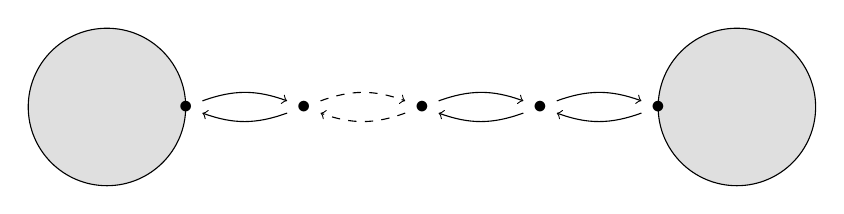
\begin{tikzpicture}

\draw[fill=lightgray!50] (-1,0) circle [radius=1];

\draw[fill=lightgray!50] (7,0) circle [radius=1];

\node (A) at (0,0) {\(\bullet\)};
\node (B) at (1.5,0) {\(\bullet\)};
\node (C) at (3,0) {\(\bullet\)};
\node (D) at (4.5,0) {\(\bullet\)};
\node (E) at (6,0) {\(\bullet\)};

\draw[->, bend left=20] (A) to (B);
\draw[->, dashed, bend left=20] (B) to (C);
\draw[->, bend left=20] (C) to (D);
\draw[->, bend left=20] (D) to (E);
\draw[->, bend left=20] (E) to (D);
\draw[->, bend left=20] (D) to (C);
\draw[->, dashed, bend left=20] (C) to (B);
\draw[->, bend left=20] (B) to (A);

\end{tikzpicture}
\caption{Sparse edge construction for the no-search scenario. The two circles represent the original dense clusters. Dashed edges have probability $\ep$.}
\label{fig1}
\end{figure}


\paragraph{Lower bounding $\SD(\calP;\MM)$.} We take an arbitrary kernel $p\in\PP$ and make the following modification, pictured in Figure \ref{fig1}. Each sparse edge $(x,y)$ is replaced by a set of states $z_0=x,z_1,\cdots,z_{q-1},z_q=y$ such that each neighboring pair $z_t,z_{t+1}$ for $t\in\ZZ_q$ are connected to each other via bidirectional edges of probability $O(1)$. However, one specific pair $z_t,z_{t+1}$ is to be connected to each other with probability $\ep$. Denote this index by $v_j$ where $j\in [J]$ numbers the set of directly connected clusters; it holds that $J=|E_s|=\Theta(K)$ by Assumption \ref{ass:sparse}. The points $z_t$ for $t\le v_j$ and for $t>v_j$ are appended to the clusters containing $x$ and $y$, respectively. Since this is a bounded number of points all connected by constant probability edges, the extended clusters are still rapidly mixing. Then each vector $v=(v_j)\in \ZZ_q^J$ determines a kernel $p_v\in \calP$, and
\begin{equation*}
\abs{E_s(p_v) \cap E_s(p_{v'})} =2(J-d_H(v,v'))
\end{equation*}
holds for all $v,v'\in\ZZ_q^J$. We now repeat the argument from before to show orthogonality: by Lemma \ref{thm:gv} there exists a $\tau J$-separated subset $\calV\subset\ZZ_q^J$ of size $A_q(J,\tau J)$ for $\tau=1-\log q/q$, and by choosing $q$ large enough we can ensure
\begin{equation*}
\abs{\MM_{p_v}(X_{\inn},X_{\out}) \cap E_s(p_v)} \ge cK > \left(\frac{2\log q}{q}\right) J \ge \abs{E_s(p_v) \cap E_s(p_{v'})}.
\end{equation*}
The key aspect of this construction is that the support of $p_v$ does not depend on $v$, as only the position of the sparse edge among $q$ candidates change with $v$. This implies that querying the path $\MM_{p_v}(X_{\inn},X_{\out})$ (and indeed the entire set of edges) does not reveal any information about the ground truth $v$, and $\{p_v:v\in\calV\}$ satisfies the conditions to compute the SQ dimension with access to $\MM$. Hence we have shown that
\begin{equation*}
\SD(\calP;\MM) \ge A_q(J,\tau J) \ge e^{\Omega(K)}.
\end{equation*}


\begin{figure}[t]
\centering
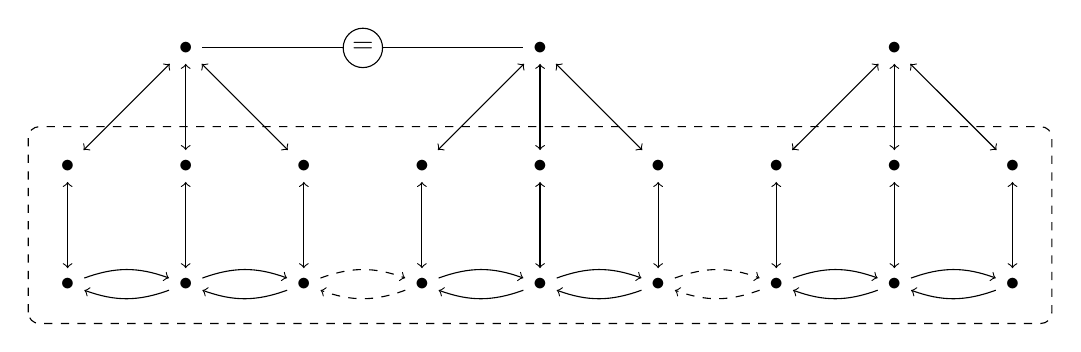
\begin{tikzpicture}

\node (A) at (0,0) {\(\bullet\)};
\node (B) at (1.5,0) {\(\bullet\)};
\node (C) at (3,0) {\(\bullet\)};
\node (D) at (4.5,0) {\(\bullet\)};
\node (E) at (6,0) {\(\bullet\)};
\node (F) at (7.5,0) {\(\bullet\)};
\node (G) at (9,0) {\(\bullet\)};
\node (H) at (10.5,0) {\(\bullet\)};
\node (I) at (12,0) {\(\bullet\)};

\node (b1) at (1.5,1.5) {\(\bullet\)};
\node (e1) at (6,1.5) {\(\bullet\)};
\node (h1) at (10.5,1.5) {\(\bullet\)};
\node (b2) at (1.5,3) {\(\bullet\)};
\node (e2) at (6,3) {\(\bullet\)};
\node (h2) at (10.5,3) {\(\bullet\)};

\node (a) at (0,1.5) {\(\bullet\)};
\node (c) at (3,1.5) {\(\bullet\)};
\node (d) at (4.5,1.5) {\(\bullet\)};
\node (f) at (7.5,1.5) {\(\bullet\)};
\node (g) at (9,1.5) {\(\bullet\)};
\node (i) at (12,1.5) {\(\bullet\)};

\draw[->, bend left=20] (A) to (B);
\draw[->, bend left=20] (B) to (C);
\draw[->, dashed, bend left=20] (C) to (D);
\draw[->, bend left=20] (D) to (E);
\draw[->, bend left=20] (E) to (F);
\draw[->, dashed, bend left=20] (F) to (G);
\draw[->, bend left=20] (G) to (H);
\draw[->, bend left=20] (H) to (I);
\draw[->, bend left=20] (I) to (H);
\draw[->, bend left=20] (H) to (G);
\draw[->, dashed, bend left=20] (G) to (F);
\draw[->, bend left=20] (F) to (E);
\draw[->, bend left=20] (E) to (D);
\draw[->, dashed, bend left=20] (D) to (C);
\draw[->, bend left=20] (C) to (B);
\draw[->, bend left=20] (B) to (A);

\draw[<->] (B) to (b1);
\draw[<->] (b1) to (b2);
\draw[<->] (E) to (e1);
\draw[<->] (e1) to (e2);
\draw[<->] (H) to (h1);
\draw[<->] (h1) to (h2);

\draw[<->] (A) to (a);
\draw[<->] (C) to (c);
\draw[<->] (D) to (d);
\draw[<->] (F) to (f);
\draw[<->] (G) to (g);
\draw[<->] (I) to (i);

\draw[<->] (a) to (b2);
\draw[<->] (c) to (b2);
\draw[<->] (d) to (e2);
\draw[<->] (f) to (e2);
\draw[<->] (g) to (h2);
\draw[<->] (i) to (h2);

\draw (b2) -- (e2);
\draw[fill=white] (3.75,3) circle (0.25);
\node at (3.75,3) {=};

\draw[dashed, rounded corners] (-0.5,-0.5) rectangle (12.5,2);

\end{tikzpicture}
\caption{Graph construction for the local search scenario ($r=2$). Dashed edges have probability $\ep$. A local neighborhood of maximum distance one from the original graph is shown in the dashed box, which the learner is assumed to have full access to.}
\label{fig2}
\end{figure}


\paragraph{Lower bounding $\SD(\calP;\nbd(\MM))$.} We construct the graph depicted in Figure \ref{fig2} as follows. We start with $nK$ clusters of size $M$ laid out in side by side and connect neighboring clusters with bidirectional edges of probability $\ep$. From all states extend a `rod' of probability $O(1)$ bidirectional edges of bounded length $r$ (the vertically arranged states, here $r=2$), similarly to Figure \ref{fig1}. Join the endpoints of all rods originating from each cluster into a single `endpoint' state. For $\DD$, we assume that $(X_{\inn},X_{\out})$ are sampled only from the original clusters (bottom horizontal line of states) and $\MM_p$ only returns paths along this line.

Choose a size $K$ subset $B$ of the low probability edges to be sparse edges, viewed as a subset of $[nK]$. For each of the edges $(x,y)$ not in $B$, identify the endpoint states of the clusters containing $x,y$. The identified clusters will merge into a single larger rapidly mixing cluster, so that $(x,y)$ is indeed no longer a sparse edge. Denote the resulting kernel as $p_B$. We have the following intersection constraint bound:
\begin{lemma}
For any $n\ge 5$, there exists a size $e^{\Omega(K)}$ set $\BB$ of size $K$ subsets of $[nK]$ such that $|B\cap B'|\le cK$ for all $B,B'\in\BB$.
\end{lemma}

\begin{proof}
We construct $\BB$ via a greedy algorithm similarly to the Gilbert-Varshamov bound. Start with $\BB=\varnothing$ and add any $B\subset[nK]$ of size $K$ not already in $\BB$ to $\BB$. Each new element blocks at most
\begin{equation*}
\binom{K}{cK}\binom{nK-cK}{K-cK}
\end{equation*}
elements from being added to $\BB$. Hence the maximum size of $\BB$ is at least
\begin{equation*}
\binom{nK}{K} \binom{K}{cK}^{-1} \binom{nK-cK}{K-cK}^{-1} = \binom{nK}{K} \binom{K}{cK}^{-2} \ge O(n^K K^{-1/2})\cdot 2^{-2K} \ge e^{\Omega(K)}
\end{equation*}
for $n\ge 5$.
\end{proof}
Then $\abs{E_s(p_B) \cap E_s(p_{B'})} = |B\cap B'| \le cK$ and we can repeat the same argument to show orthogonality. Furthermore by taking $r$ sufficiently large, the local neighborhood of any path contained in the bottom horizontal line (which must be contained in the dashed area in Figure \ref{fig2}) is isomorphic for all $B\in\BB$, since it cannot query the endpoint states to identify which clusters are actually connected. Hence $\{p_B:B\in\BB\}$ satisfies the conditions to compute the SQ
dimension with access to $\nbd(\MM)$, and thus
\begin{equation*}
\SD(\calP;\nbd(\MM)) \ge |\BB| \ge e^{\Omega(K)}.
\end{equation*}
\qed
